\chapter{Aplicaciones informáticas}


En este capítulo se describen las aplicaciones informáticas que se han desarrollado como complemento a las ideas que se exponen a lo largo del trabajo y que servirán de gran ayuda para visualizar los resultados que se exponen. \\

Se han desarrollado dos aplicaciones en Python. La primera de ellas permite generar el coloreado de las funciones complejas en un disco de radio arbitrario mientras que la segunda permite extender una función $f: \partial \disk \to \complex$ al disco unidad abierto con continuidad. Para producir el coloreado de ambas aplicaciones se utiliza la técnica de visualización de las funciones complejas conocida como coloreado del dominio. \\

% Con ello se pretende que se pueda utilizar en docencia, tanto profesores como estudiantes. Y estos, en particular, para desarrollar su intuición o conjeturar sobre problemas concretos (naturaleza de singularidades aisladas, orden de los polos, multiplicidad de los ceros, etc.). \\

\section{Técnica del coloreado del dominio}

En esta sección se presentan técnicas de visualización de las funciones complejas que permiten resaltar algunas propiedades geométricas que poseen tales como  ... \\

A la hora de reflejar el comportamiento de funciones complejas, inmediatamente tenemos que lidiar con una dificultad implícita: los números complejos son bidimensionales, así que el grafo de una función $f : \complex \to \complex$, requerirá de cuatro dimensiones. La solución que propone \cite{Velleman2015} y que se va a emplear para representar estas funciones a lo largo del texto es la asignación de un color a cada número complejo. Esta forma de representación se denomina \textbf{Coloreado del dominio} (en inglés \textit{Domain Coloring}). \\

Por lo tanto, la técnica del coloreado consiste en asignar a cada número complejo un determinado color que depende de su módulo y su argumento. La figura \ref{fig:z} muestra el plano complejo en el que a cada punto se le ha asignado un color distinto, de acuerdo al procedimiento que se describe a continuación. \\

En cuanto al argumento, conforme vamos aumentando el argumento el color va variando de rojo, amarillo, verde, cyan, azul, magenta y volviendo de nuevo al rojo. Según esta asignación, los puntos puramente reales se corresponden con el rojo en el eje positivo mientras que en el eje negativo se corresponden con el cyan. \\

En cuanto al módulo, los puntos cercanos al origen se corresponden con colores oscuros mientras que los puntos alejados tienen colores claros. Así, cuando $\abs{z}$ tiende a $0$, el color asignado se acerca al negro, en cambio cuando $\abs{z}$ tiende a infinito, el color de $z$ se aproxima al blanco. \\

Con esta representación, cada número complejo tiene asignado un color diferente, por lo que un número complejo puede especificarse de manera única por su color. Así que podemos representar cualquier función $f : \complex \to \complex$ de la siguiente manera: a cada punto $z$ se le asigna el color correspondiente a $f(z)$. De este modo, se representa cualquier función compleja en dos dimensiones con los colores, tomando como referencia la figura \ref{fig:z}, que representa la función identidad $f(z) = z$. \\

\begin{figure}[h]
    \centering
    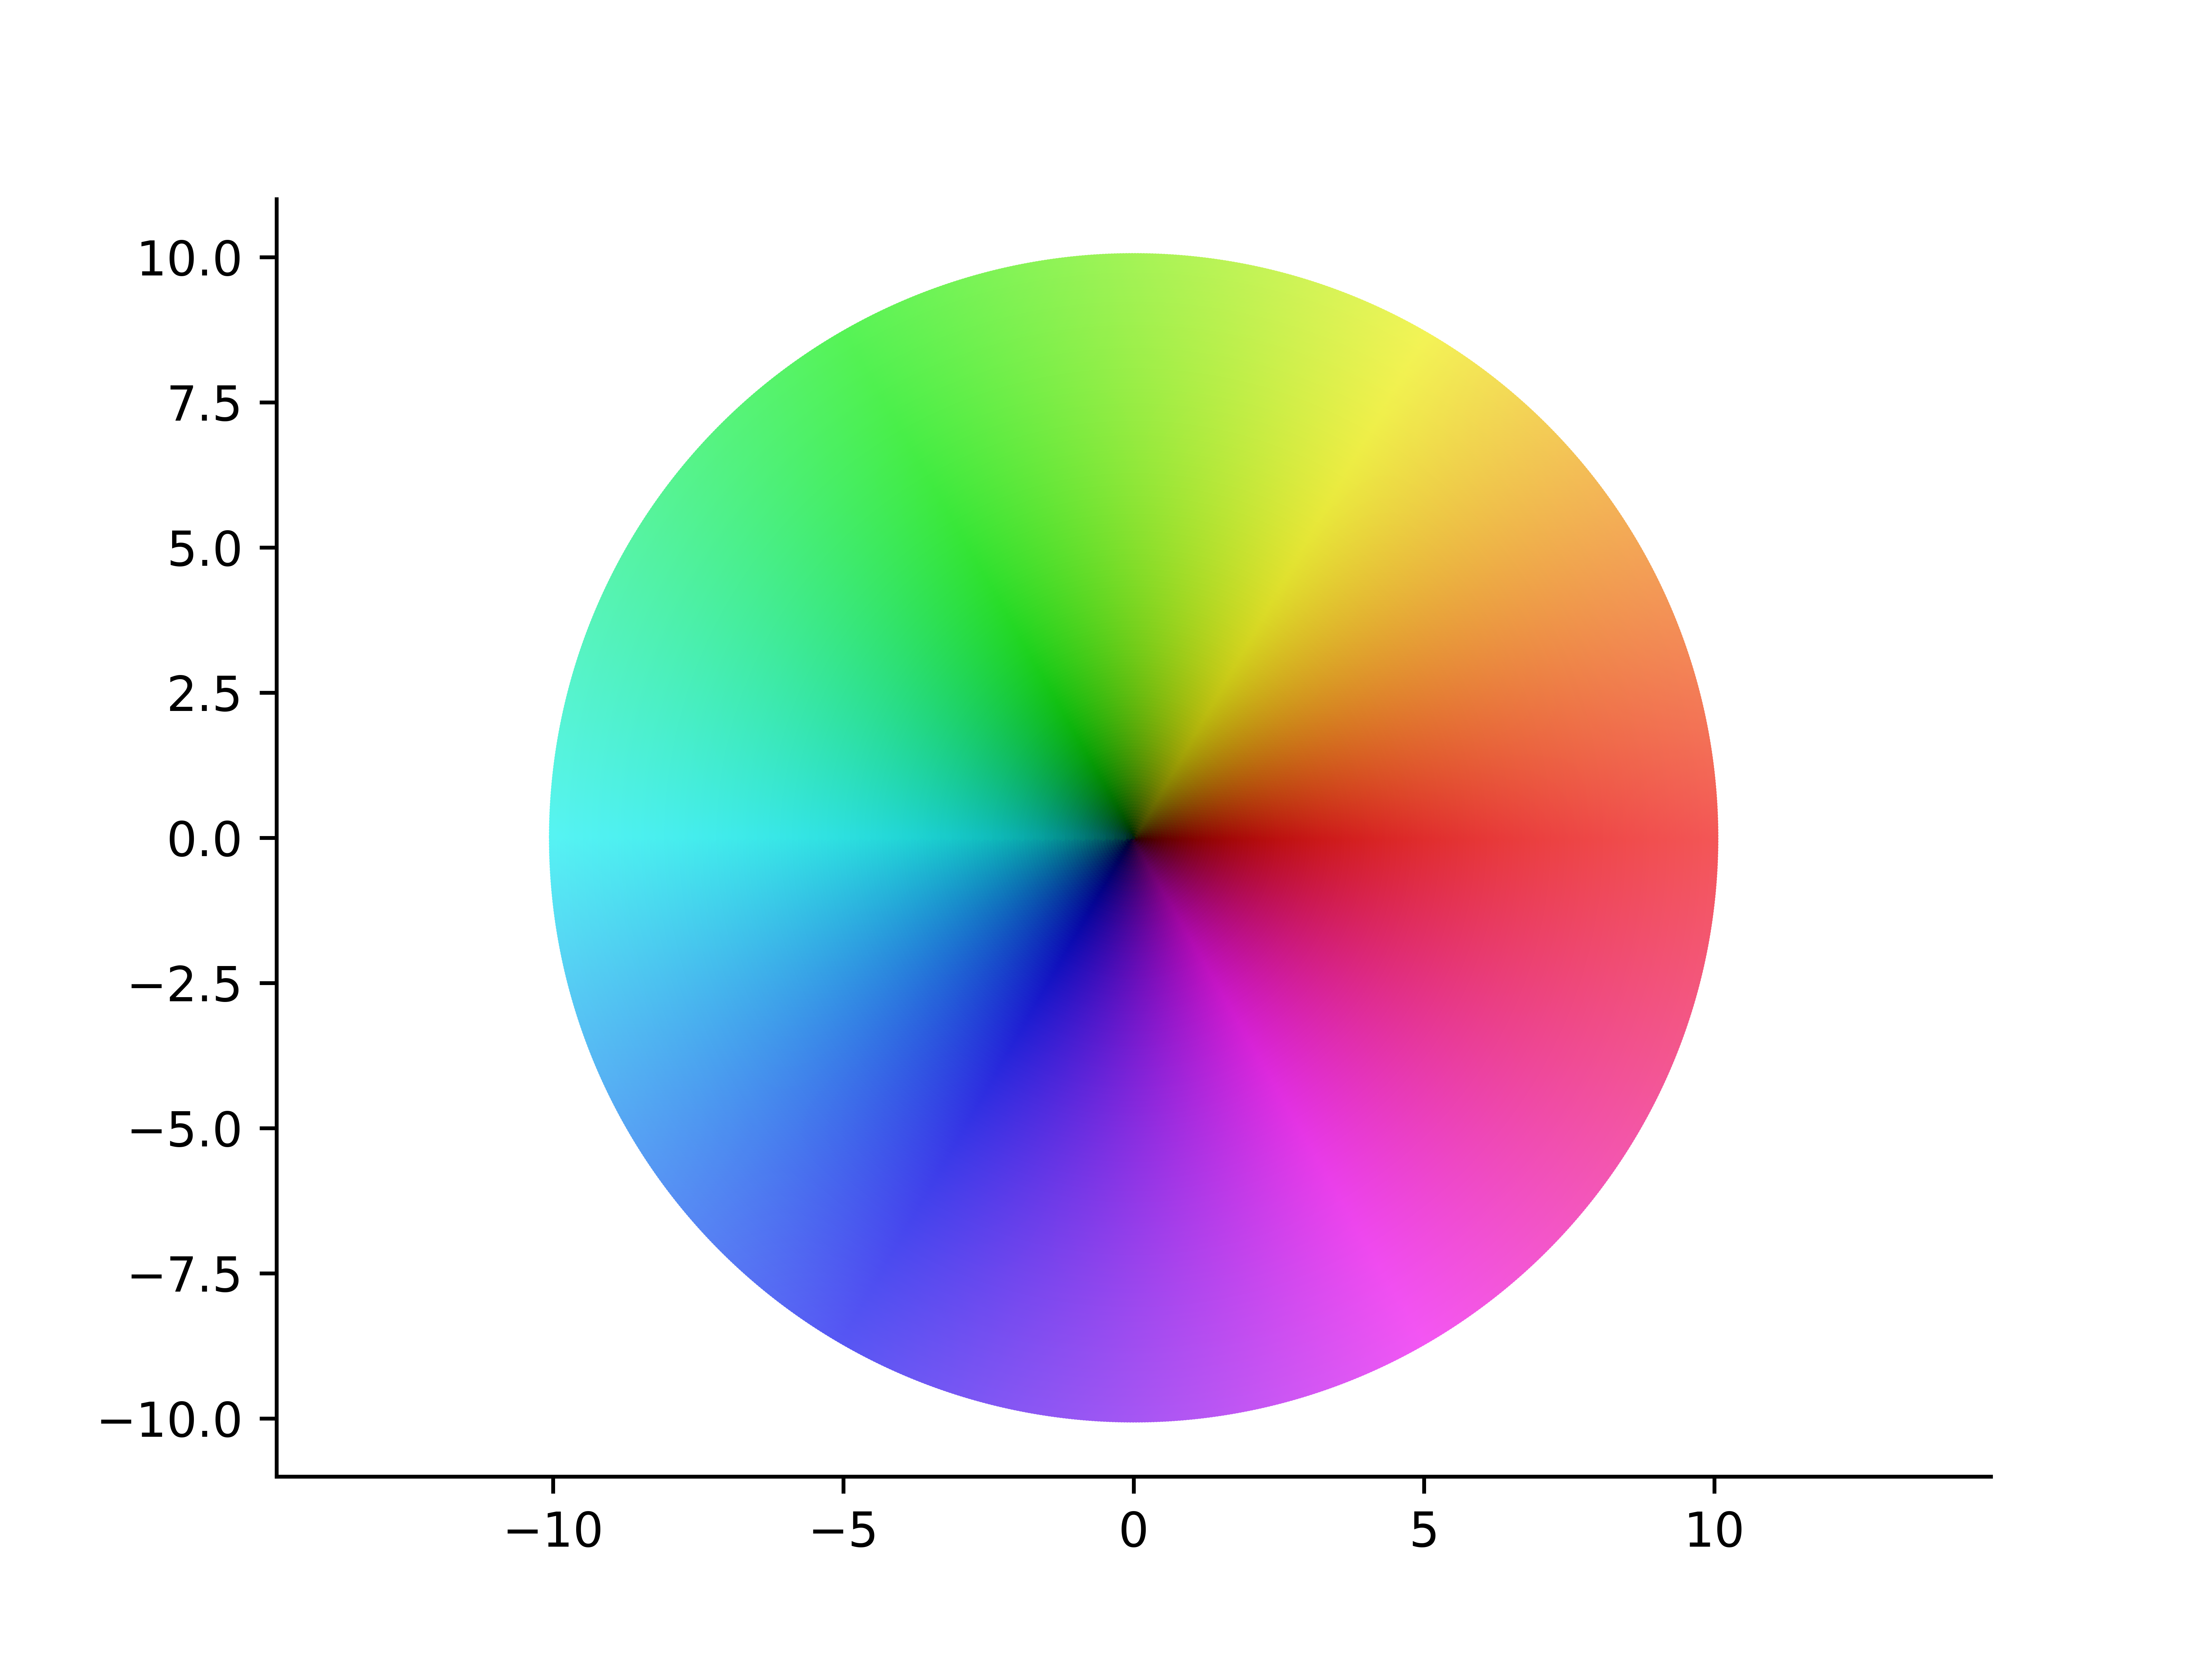
\includegraphics[width=0.7\textwidth]{../Aplicacion/z.png}
    \caption{Plano complejo coloreado}
    \label{fig:z}
\end{figure}

A continuación mostramos con un ejemplo la gran cantidad de información que podemos extraer gracias a la representación de funciones complejas mediante la técnica de coloreado del dominio. \\

La figura \ref{fig:z^8-2z^7+2z^6-4z^5+2z^4-2z^3-5z^2+4z-4} es la representación de la función $f(z) = z^8-2z^7+2z^6-4z^5+2z^4-2z^3-5z^2+4z-4$ mediante la técnica del coloreado. Puesto que el color asignado al número $0$ es el negro, las raíces de $f$ vienen representadas por los $6$ puntos negros en el dibujo. Sin embargo, este polinomio tiene $8$ raíces de las cuales $2$ son raíces dobles. Las raíces simples ocurren en los puntos $-1$, $2$ y $\frac{(-1 \rpm i \sqrt{7})}{2}$, y las raíces dobles en $\frac{1 \rpm i \sqrt{3}}{2}$.  La región que rodea a las raíces dobles es algo más oscura que la que rodea a las raíces simples, y en las raíces dobles los colores del círculo cromático la envuelven dos veces, mientras que en las raíces simples la envuelven una sola vez. \\

Además, el dibujo también muestra que el polinomio es de grado $8$. Para $z$ de módulo grande, el término de $z^8$ domina a los otros términos, y por consiguiente la parte exterior del dibujo es similar a la representación de la función $z^8$. Esto puede observarse en que los colores del círculo cromático aparecen ocho veces. \\

\begin{figure}[h]
    \centering
    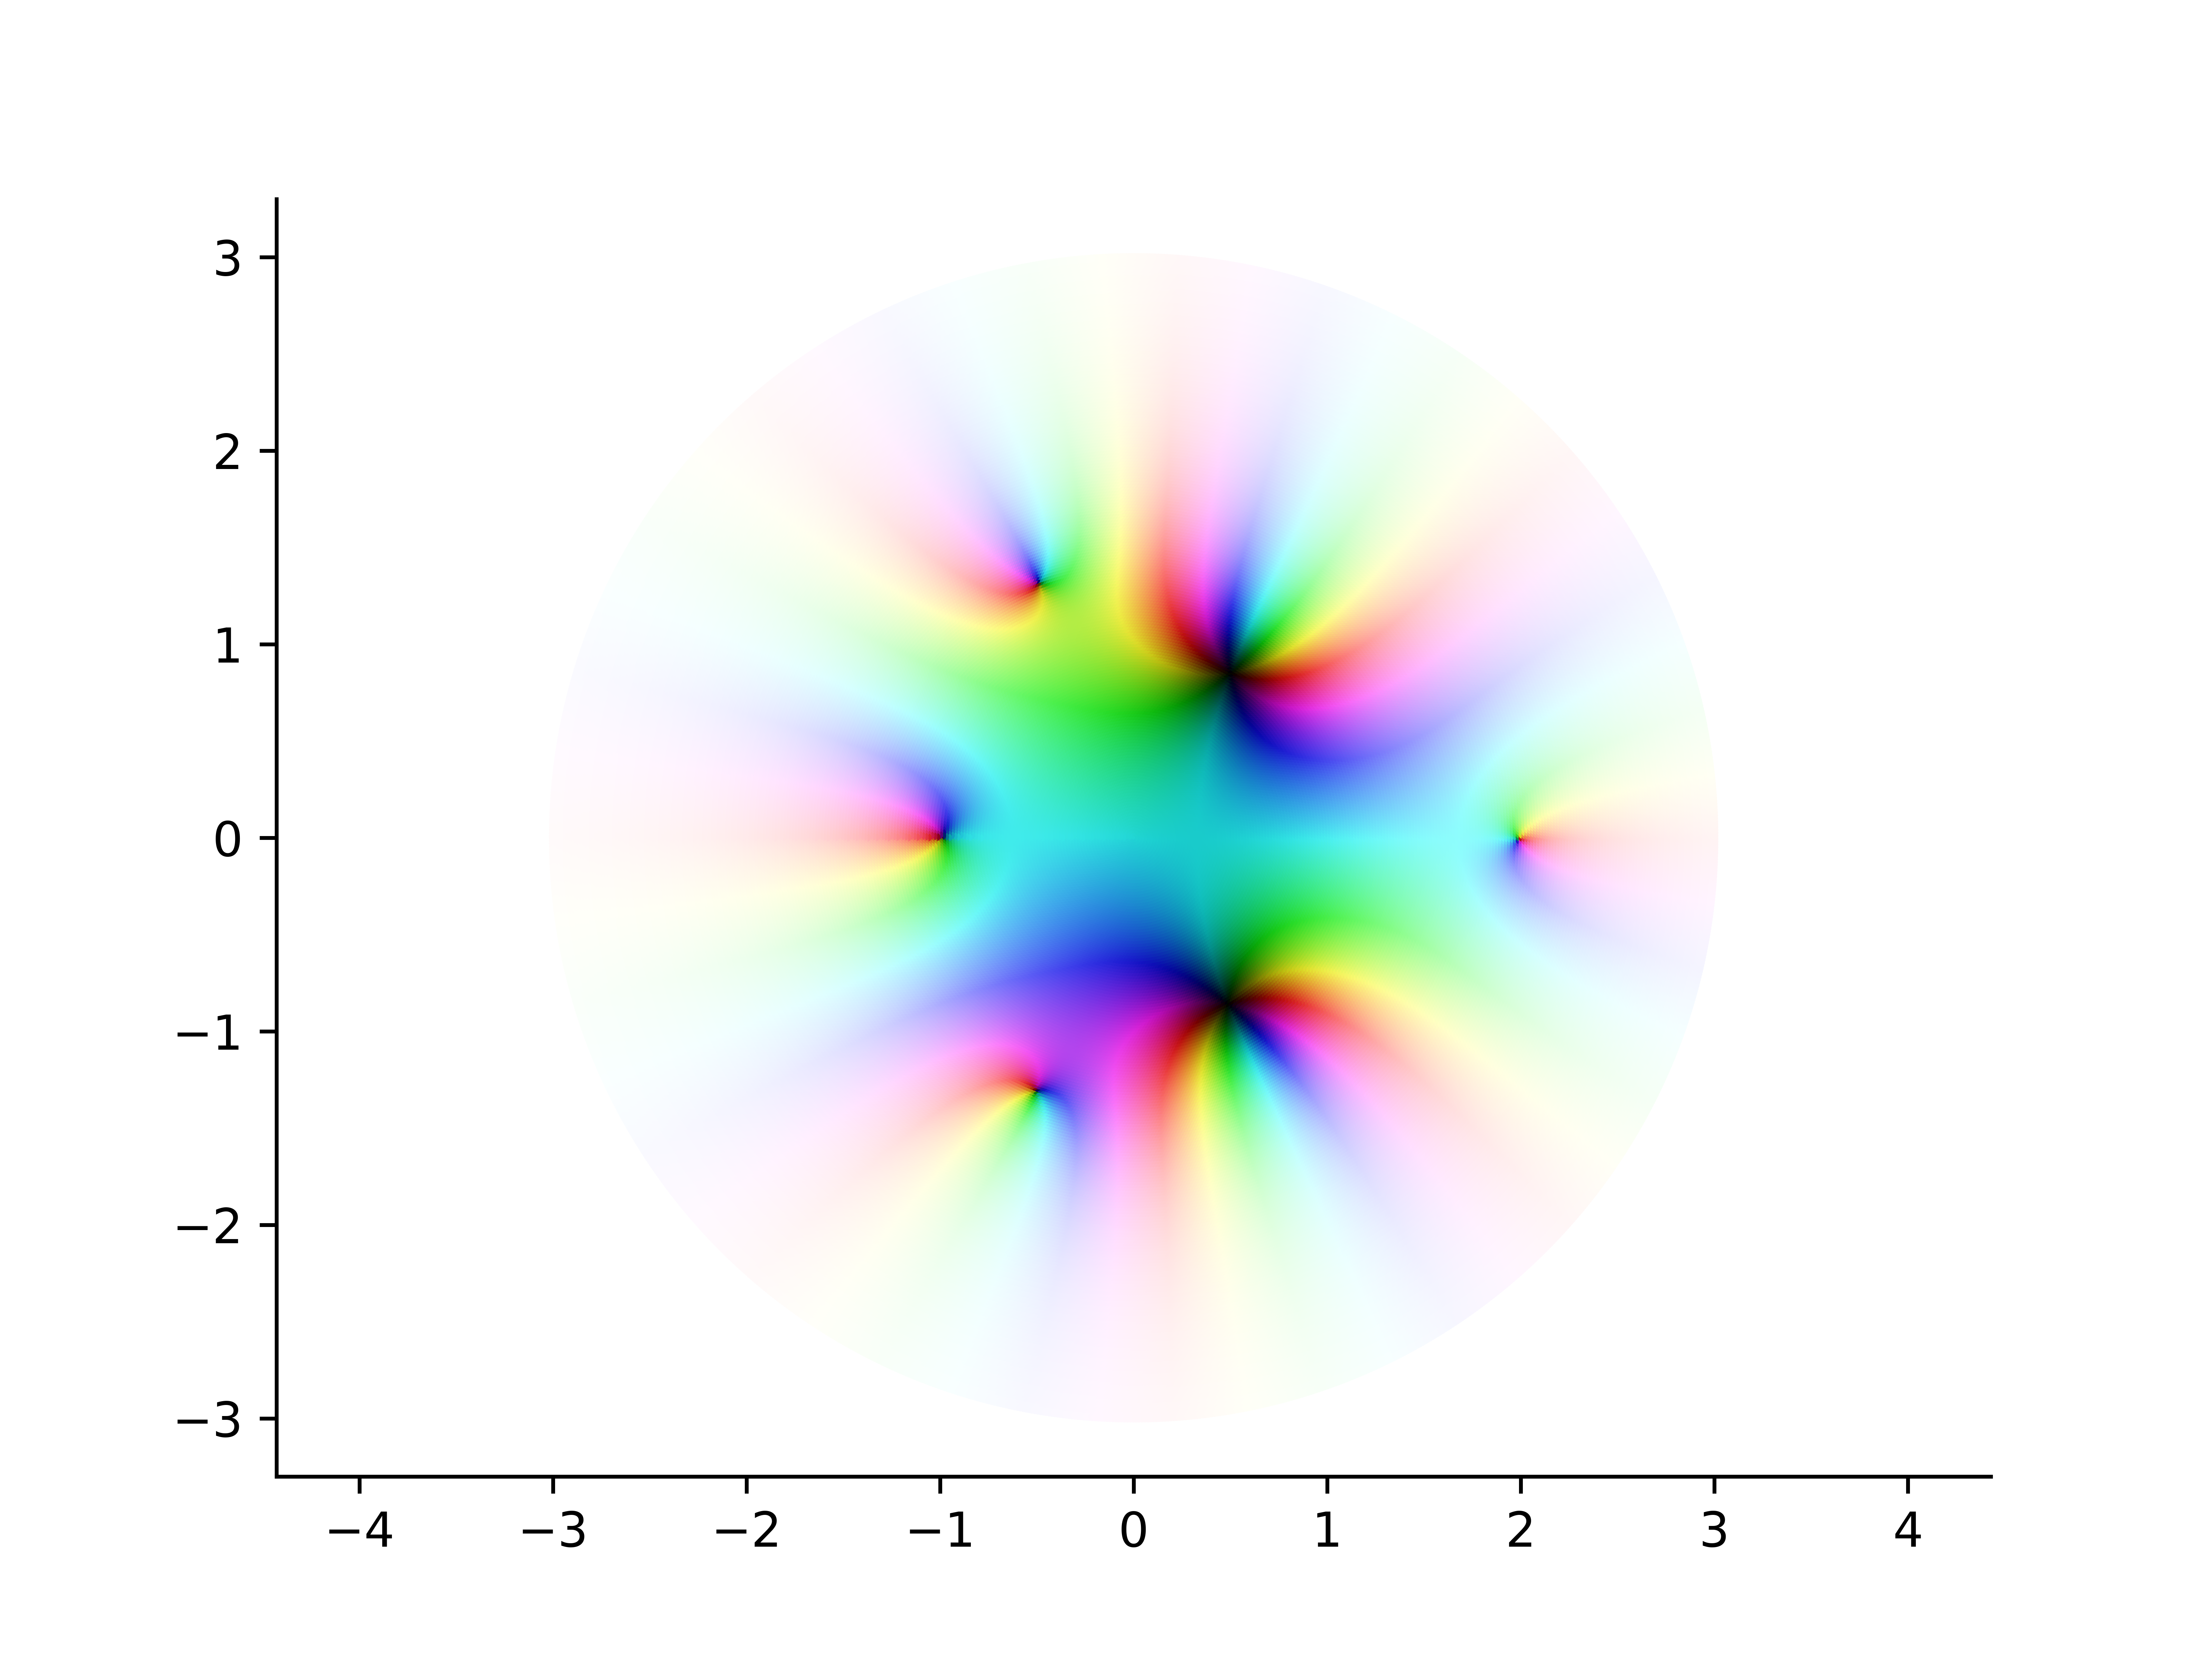
\includegraphics[width=0.7\textwidth]{../Aplicacion/z^8-2z^7+2z^6-4z^5+2z^4-2z^3-5z^2+4z-4.png}
    \caption{$f(z) = z^8-2z^7+2z^6-4z^5+2z^4-2z^3-5z^2+4z-4$}
    \label{fig:z^8-2z^7+2z^6-4z^5+2z^4-2z^3-5z^2+4z-4}
\end{figure}

%Este esquema de asignación de colores puede representarse fácilmente siguiendo el modelo de color HVS (del inglés, \textit{Hue, Saturation, Value} - Tono, Saturación, Valor).

Introducimos un modelo de color gracias al cual vamos a poder representar fácilmente funciones complejas siguiendo el esquema de asignación de colores explicado anteriormente. Dicho modelo se conoce como HVS (del inglés, \textit{Hue, Saturation, Value} - Tono, Saturación, Valor). \\

El primero de los atributos, que determina el tono de un color, se puede especificar por el ángulo que ocupa alrededor de un punto. Según va aumentando el ángulo, el color va variando de rojo, amarillo, verde, cyan, azul, magenta para volver de nuevo al rojo. Así pues el tono asociado a un número complejo está directamente relacionado con su argumento. La saturación es la intensidad de un tono específico, basándose en la pureza del color: un color muy saturado es vivo e intenso, mientras que un color menos saturado es más descolorido y gris. Por último, el valor indica la cantidad de luz que tiene un color. Cuánto más oscuro sea, menor será su valor y cuánto más claro, mayor. De este modo, la saturación y el valor asociadas a un número complejo están relacionados con el módulo del mismo. \\

\begin{comment}
\begin{figure}[h]{}
    \begin{minipage}[h]{0.3\textwidth}
        \centering
        \begin{tikzpicture}[scale=0.5]
        \foreach \x in {0,0.0111,...,1}{
            \definecolor{currentcolor}{hsb}{\x, 1, 1}
            \draw[draw=none, fill=currentcolor]
                (-360*\x+88:2) -- (-360*\x+88:3.8)
                -- (-360*\x+92:3.8) -- (-360*\x+92:2) -- cycle;
        }
        \end{tikzpicture}
        \label{fig:hue}
        %\caption{Tono}
    \end{minipage} \hfill
    \begin{minipage}[h]{0.3\textwidth}
        \centering
        \begin{tikzpicture}[scale=0.5]
        \foreach \x in {0,0.0111,...,1}{
            \definecolor{currentcolor}{hsb}{1, \x, 1}
            \draw[draw=none, fill=currentcolor]
                (-360*\x+88:2) -- (-360*\x+88:3.8)
                -- (-360*\x+92:3.8) -- (-360*\x+92:2) -- cycle;
        }
        \end{tikzpicture}
        \label{fig:saturation}
        %\caption{Saturación}
    \end{minipage} \hfill
    \begin{minipage}[h]{0.3\textwidth}
        \centering
        \begin{tikzpicture}[scale=0.5]
        \foreach \x in {0,0.0111,...,1}{
            \definecolor{currentcolor}{hsb}{1, 1, \x}
            \draw[draw=none, fill=currentcolor]
                (-360*\x+88:2) -- (-360*\x+88:3.8)
                -- (-360*\x+92:3.8) -- (-360*\x+92:2) -- cycle;
        }
        \end{tikzpicture}
        \label{fig:value}
        %\caption{Valor}
    \end{minipage}
    \caption{Tono, saturación y valor}
    \label{fig:hsv}
\end{figure}
\end{comment}

\begin{figure}[h]{}
    \begin{minipage}[h]{\textwidth}
        \centering
        \parbox[c][1cm]{\textwidth}{\centering \textbf{Tono}: \\}
        \begin{tikzpicture}[x=1mm,y=1mm]
            \foreach \x in {0,0.0111,...,1}{
                \definecolor{colorhsb}{hsb}{\x, 1, 1}
                \draw[fill=colorhsb, draw=none] (\x*100,1) rectangle +(1mm,7mm);
            }
            \node[below] at (0,1){$0º$};
            \node[below] at (100,1){$360º$};
        \end{tikzpicture}
        \label{fig:hue}
        %\caption{Tono}
    \end{minipage}
    \begin{minipage}[h]{\textwidth}
        \centering
        \parbox[c][1cm]{\textwidth}{}{\centering \textbf{Saturación}: \\}
        \begin{tikzpicture}[x=1mm,y=1mm]
            \foreach \x in {0,0.0111,...,1}{
                \definecolor{colorhsb}{hsb}{1, \x, 1}
                \draw[fill=colorhsb, draw=none] (\x*100,1) rectangle +(1mm,7mm);
            }
            \node[below] at (0,1){$0º$};
            \node[below] at (100,1){$100º$};
        \end{tikzpicture}
        \label{fig:saturation}
        %\caption{Saturación}
    \end{minipage}
    \begin{minipage}[h]{\textwidth}
        \centering
        \parbox[c][1cm]{\textwidth}{\centering \textbf{Valor}: \\}
        \begin{tikzpicture}[x=1mm,y=1mm]
            \foreach \x in {0,0.0111,...,1}{
                \definecolor{colorhsb}{hsb}{1, 1, \x}
                \draw[fill=colorhsb, draw=none] (\x*100,1) rectangle +(1mm,7mm);
            }
            \node[below] at (0,1){$0º$};
            \node[below] at (100,1){$100º$};
        \end{tikzpicture}
        \label{fig:value}
        %\caption{Valor}
    \end{minipage}
    \caption{Modelo de color HSV}
    \label{fig:hsv}
\end{figure}

Los colores en Python se pueden dibujar mediante tuplas RGB de valores comprendidos entre el cero y el uno, esto es, $color \, rgb = (r, g, b)$, con $0 \leq r, g, b \leq 1$. Cada uno de estos números se corresponde con uno de los tres colores primarios: rojo (\textit{red}), verde (\textit{green}) y azul (\textit{blue}). Estos colores se representan como: $rojo = (1, 0, 0)$, $verde = (0, 1, 0)$ y $azul = (0, 0, 1)$. Además, el blanco y el negro suponen todos estos valores a cero o a uno ($blanco = (1, 1, 1)$ y $negro = (0, 0, 0)$). \\

Ahora bien, Python también admite una representación de colores por medio de tuplas HSV con valores entre el cero y el uno, es decir, $color \, hsv = (h, s, v)$, con $0 \leq h, s, v \leq 1$. Así que podremos asociar a cada número complejo una terna en el modelo de colores HSV, cuidándonos de que los valores estén dentro del rango adecuado. Además, gracias a una función de Python podemos transformar directamente un color del modelo HSV en RGB. \\

De esta manera podremos representar cualquier color en Python como combinación de su tono, saturación y brillo, que dependen a su vez del módulo y el argumento del número complejo. \\

% Al hacer pruebas con diversas funciones, se ha observado que en los puntos cercanos a las raíces de las funciones su módulo es muy pequeño, pero que rápidamente se dispara en los extremos de los intervalos. Por eso se ha decidido ajustar el color del módulo de forma que los tonos oscuros los tomen los números cuyo módulo está comprendido entre cero y uno, y se toman los tonos claros entre los módulos uno y el valor del radio. \\

\section{Representación de funciones. Problema de Dirichlet}

A lo largo del trabajo nos vamos a centrar en el comportamiento de funciones en el borde del disco unidad. Por ello, la representación de funciones se realiza en discos centrados en $0$ de radio arbitrario, siendo $1$ el valor por defecto. La idea es tomar un mallado circular y evaluar la función en cada punto. \\

La aplicación que se ha desarrollado tiene tres funcionalidades diferentes. En primer lugar, permite representar funciones complejas en un disco de radio determinado, como ya se ha mostrado en las figuras \ref{fig:z} y \ref{fig:z^8-2z^7+2z^6-4z^5+2z^4-2z^3-5z^2+4z-4}, cuyos dibujos han sido obtenidos al ejecutar el programa realizado. \\

Por otra parte, también se puede resolver el problema de Dirichlet para el disco haciendo uso de la integral de Poisson. Dada una función $f$ continua definida en el borde del disco, la solución dada por la integral de Poisson será una función continua en el disco cerrado y armónica en el disco abierto. \\

La función $f$ que recibe el programa parametriza el borde del disco en función del argumento. Así pues, para poder definir funciones con mayor facilidad, su dominio de definición es $[-\pi, \pi]$ de manera que $\theta \in [-\pi, \pi]$ se corresponde con el punto $z = e^{i \theta} = \cos(\theta) + i \sen(\theta) \in \complex$. \\

Podemos utilizar la representación de funciones que se ha desarrollado para comprobar que la integral de Poisson se comporta como se espera cuando la parametrización dada se corresponde, en el borde, con la función que se va a dibujar. A continuación se pueden observar algunos ejemplos. \\

\begin{figure}[h]
    \centering
    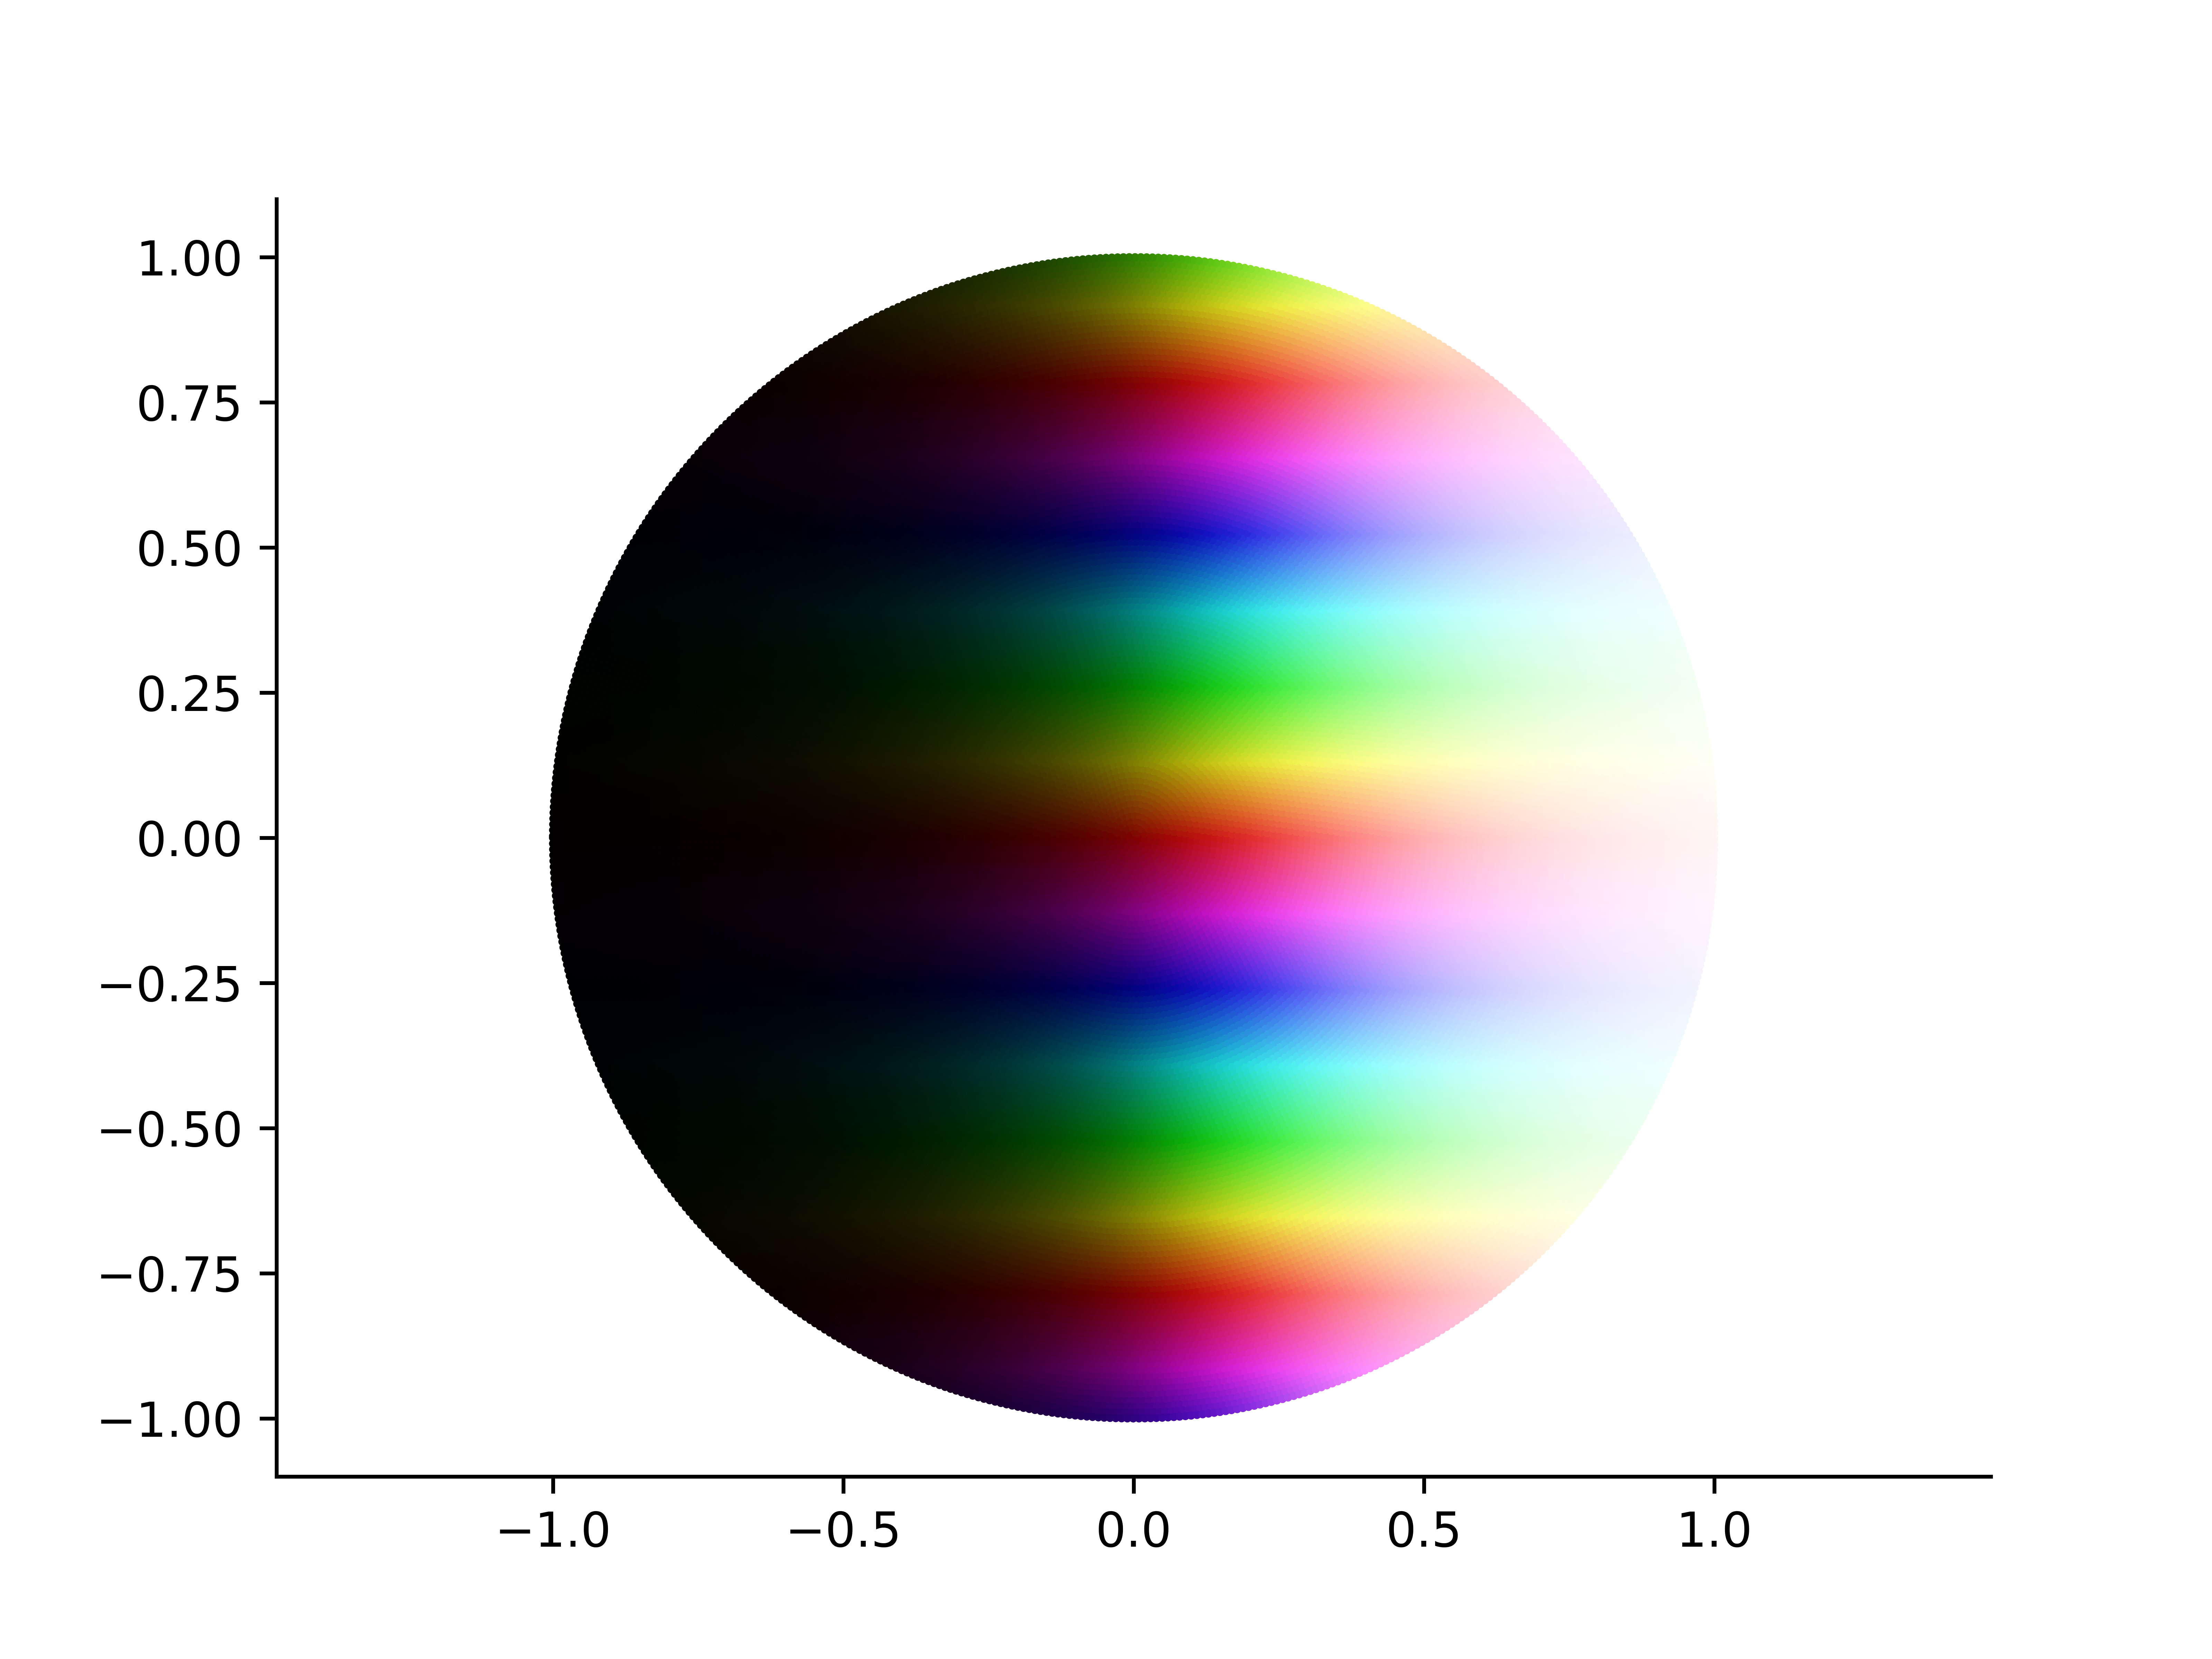
\includegraphics[width=0.49\textwidth]{../Aplicacion/e^(8z).png}
    \hfill
    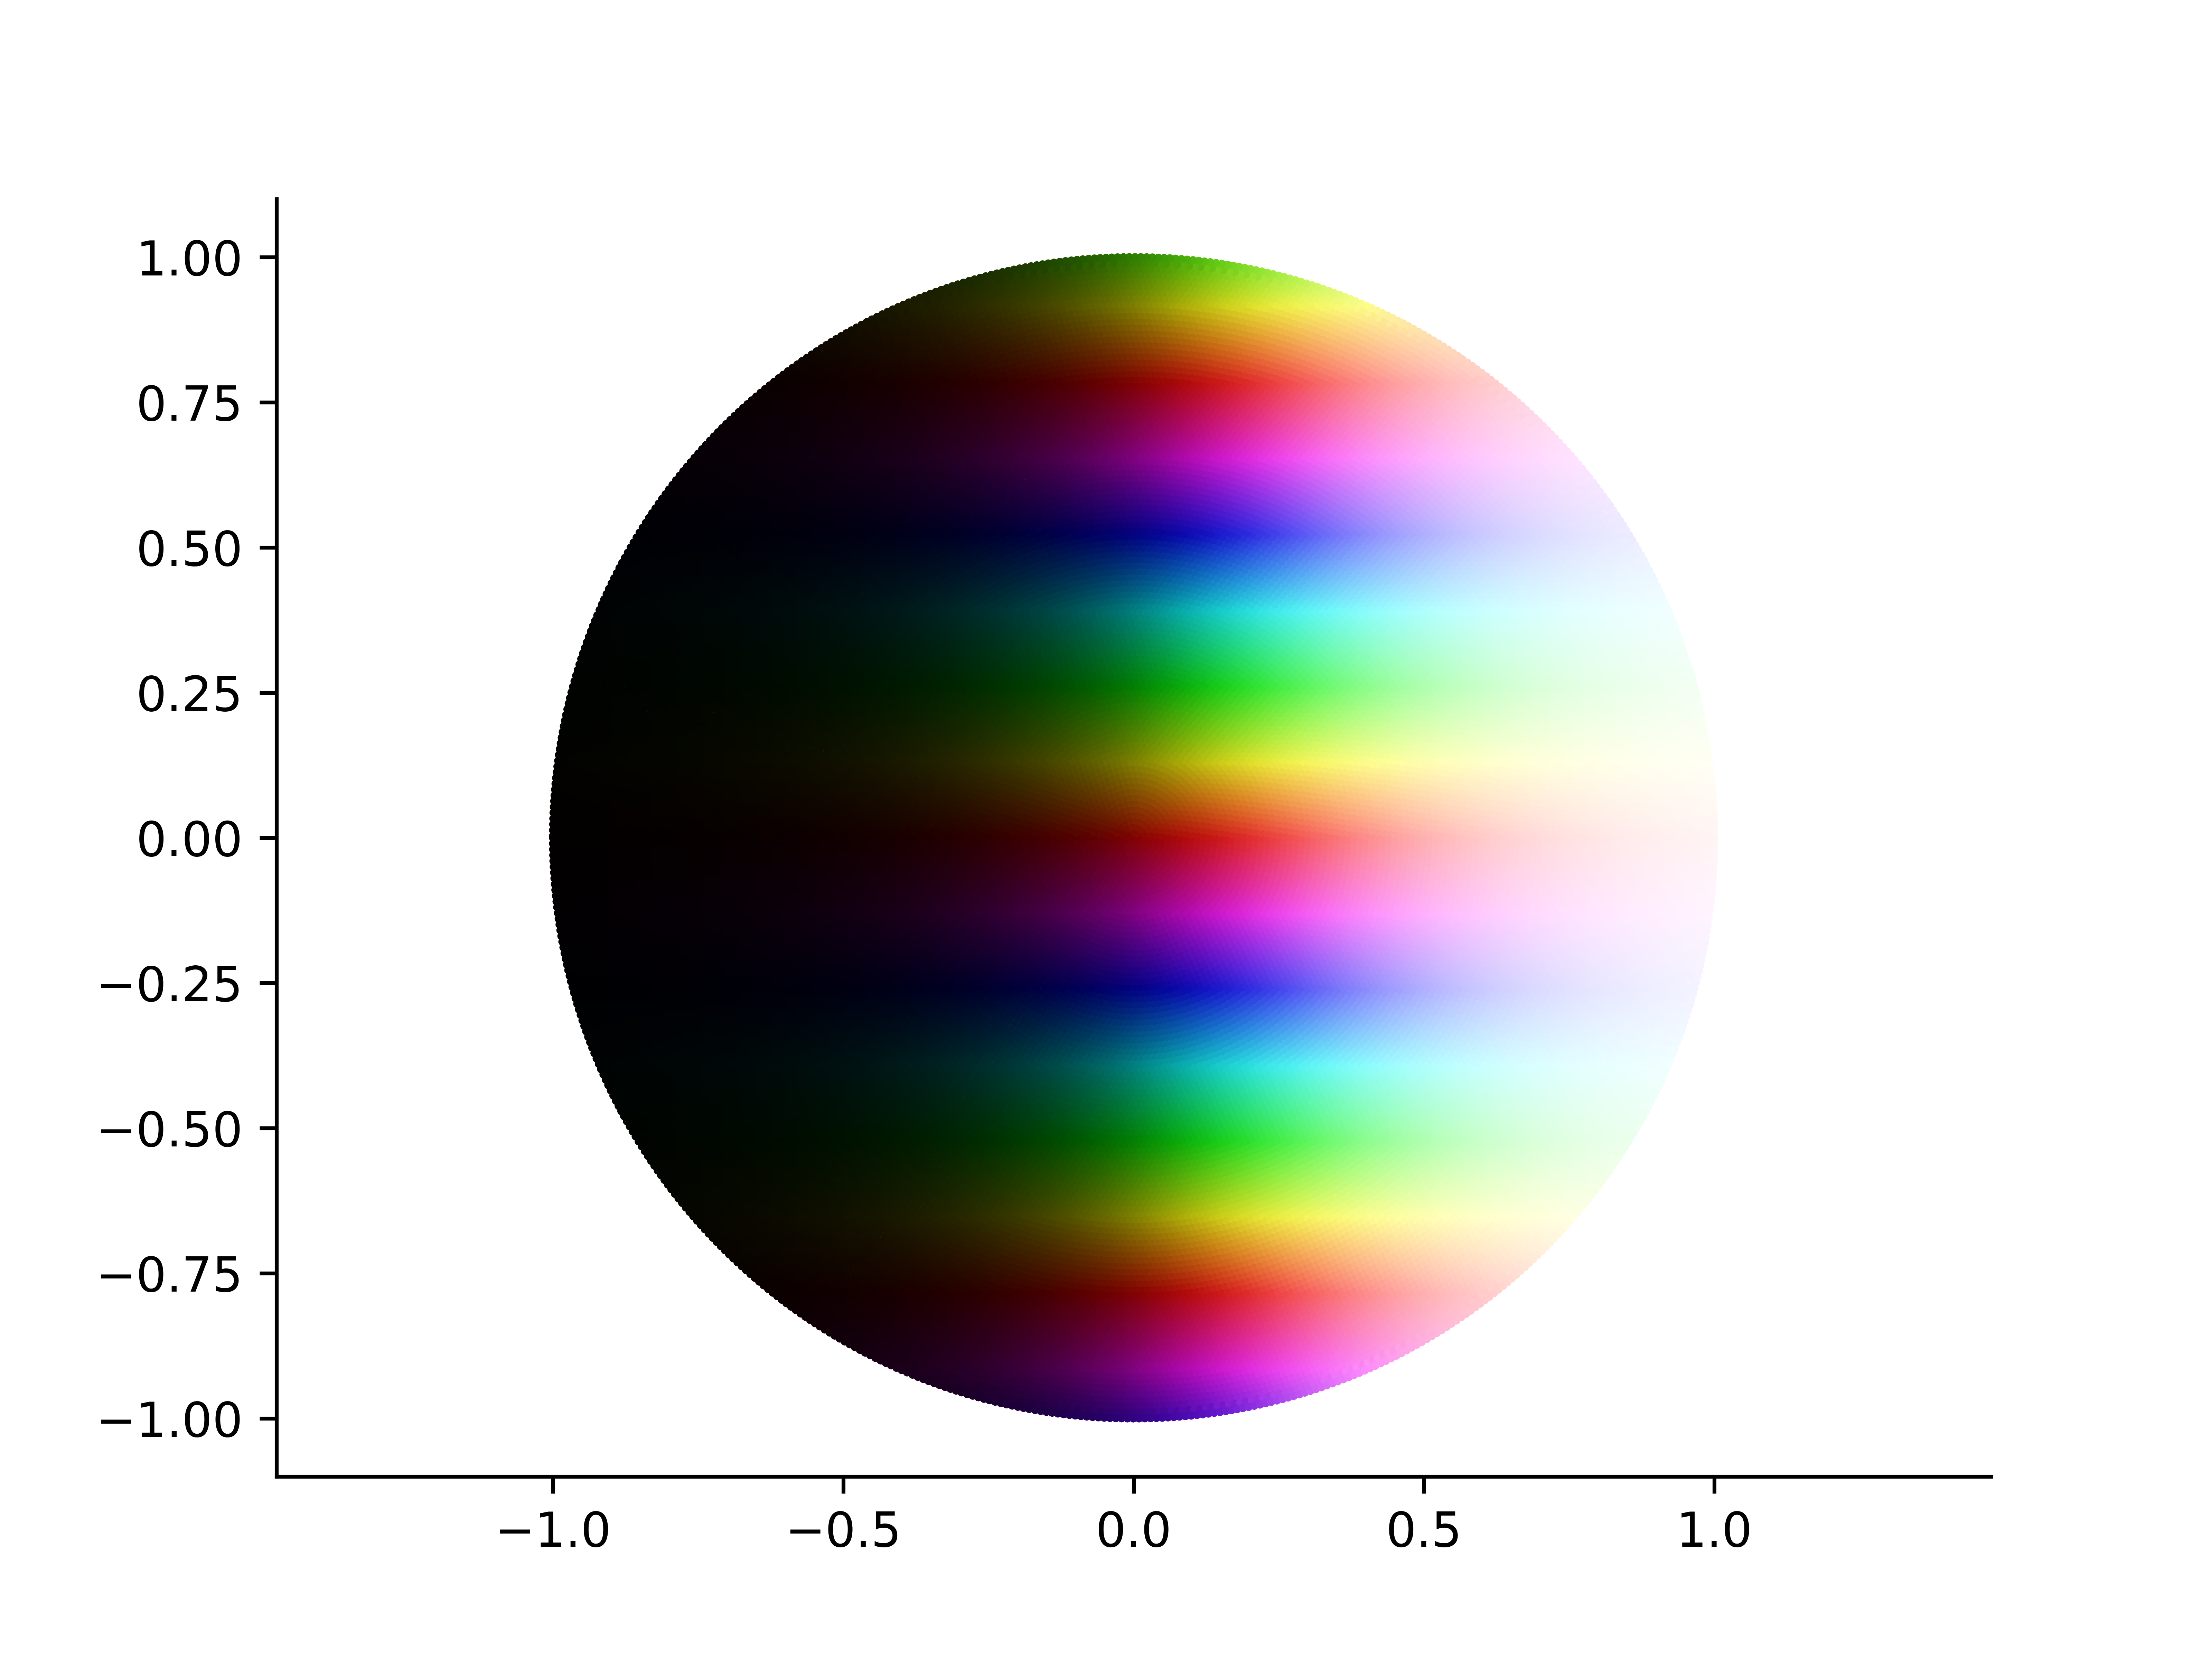
\includegraphics[width=0.49\textwidth]{../Aplicacion/e^(8cos(t)+8isen(t)).png}
    \caption{A la izquierda se muestra la representación de la función $f(z) = e^{8z}$; a la derecha se muestra la extensión al disco de la función $f(t) = e^{8 \cos(t)+8i \sen(t)}$.}
    \label{fig:comparacion1}
\end{figure}

\begin{figure}[h]
    \centering
    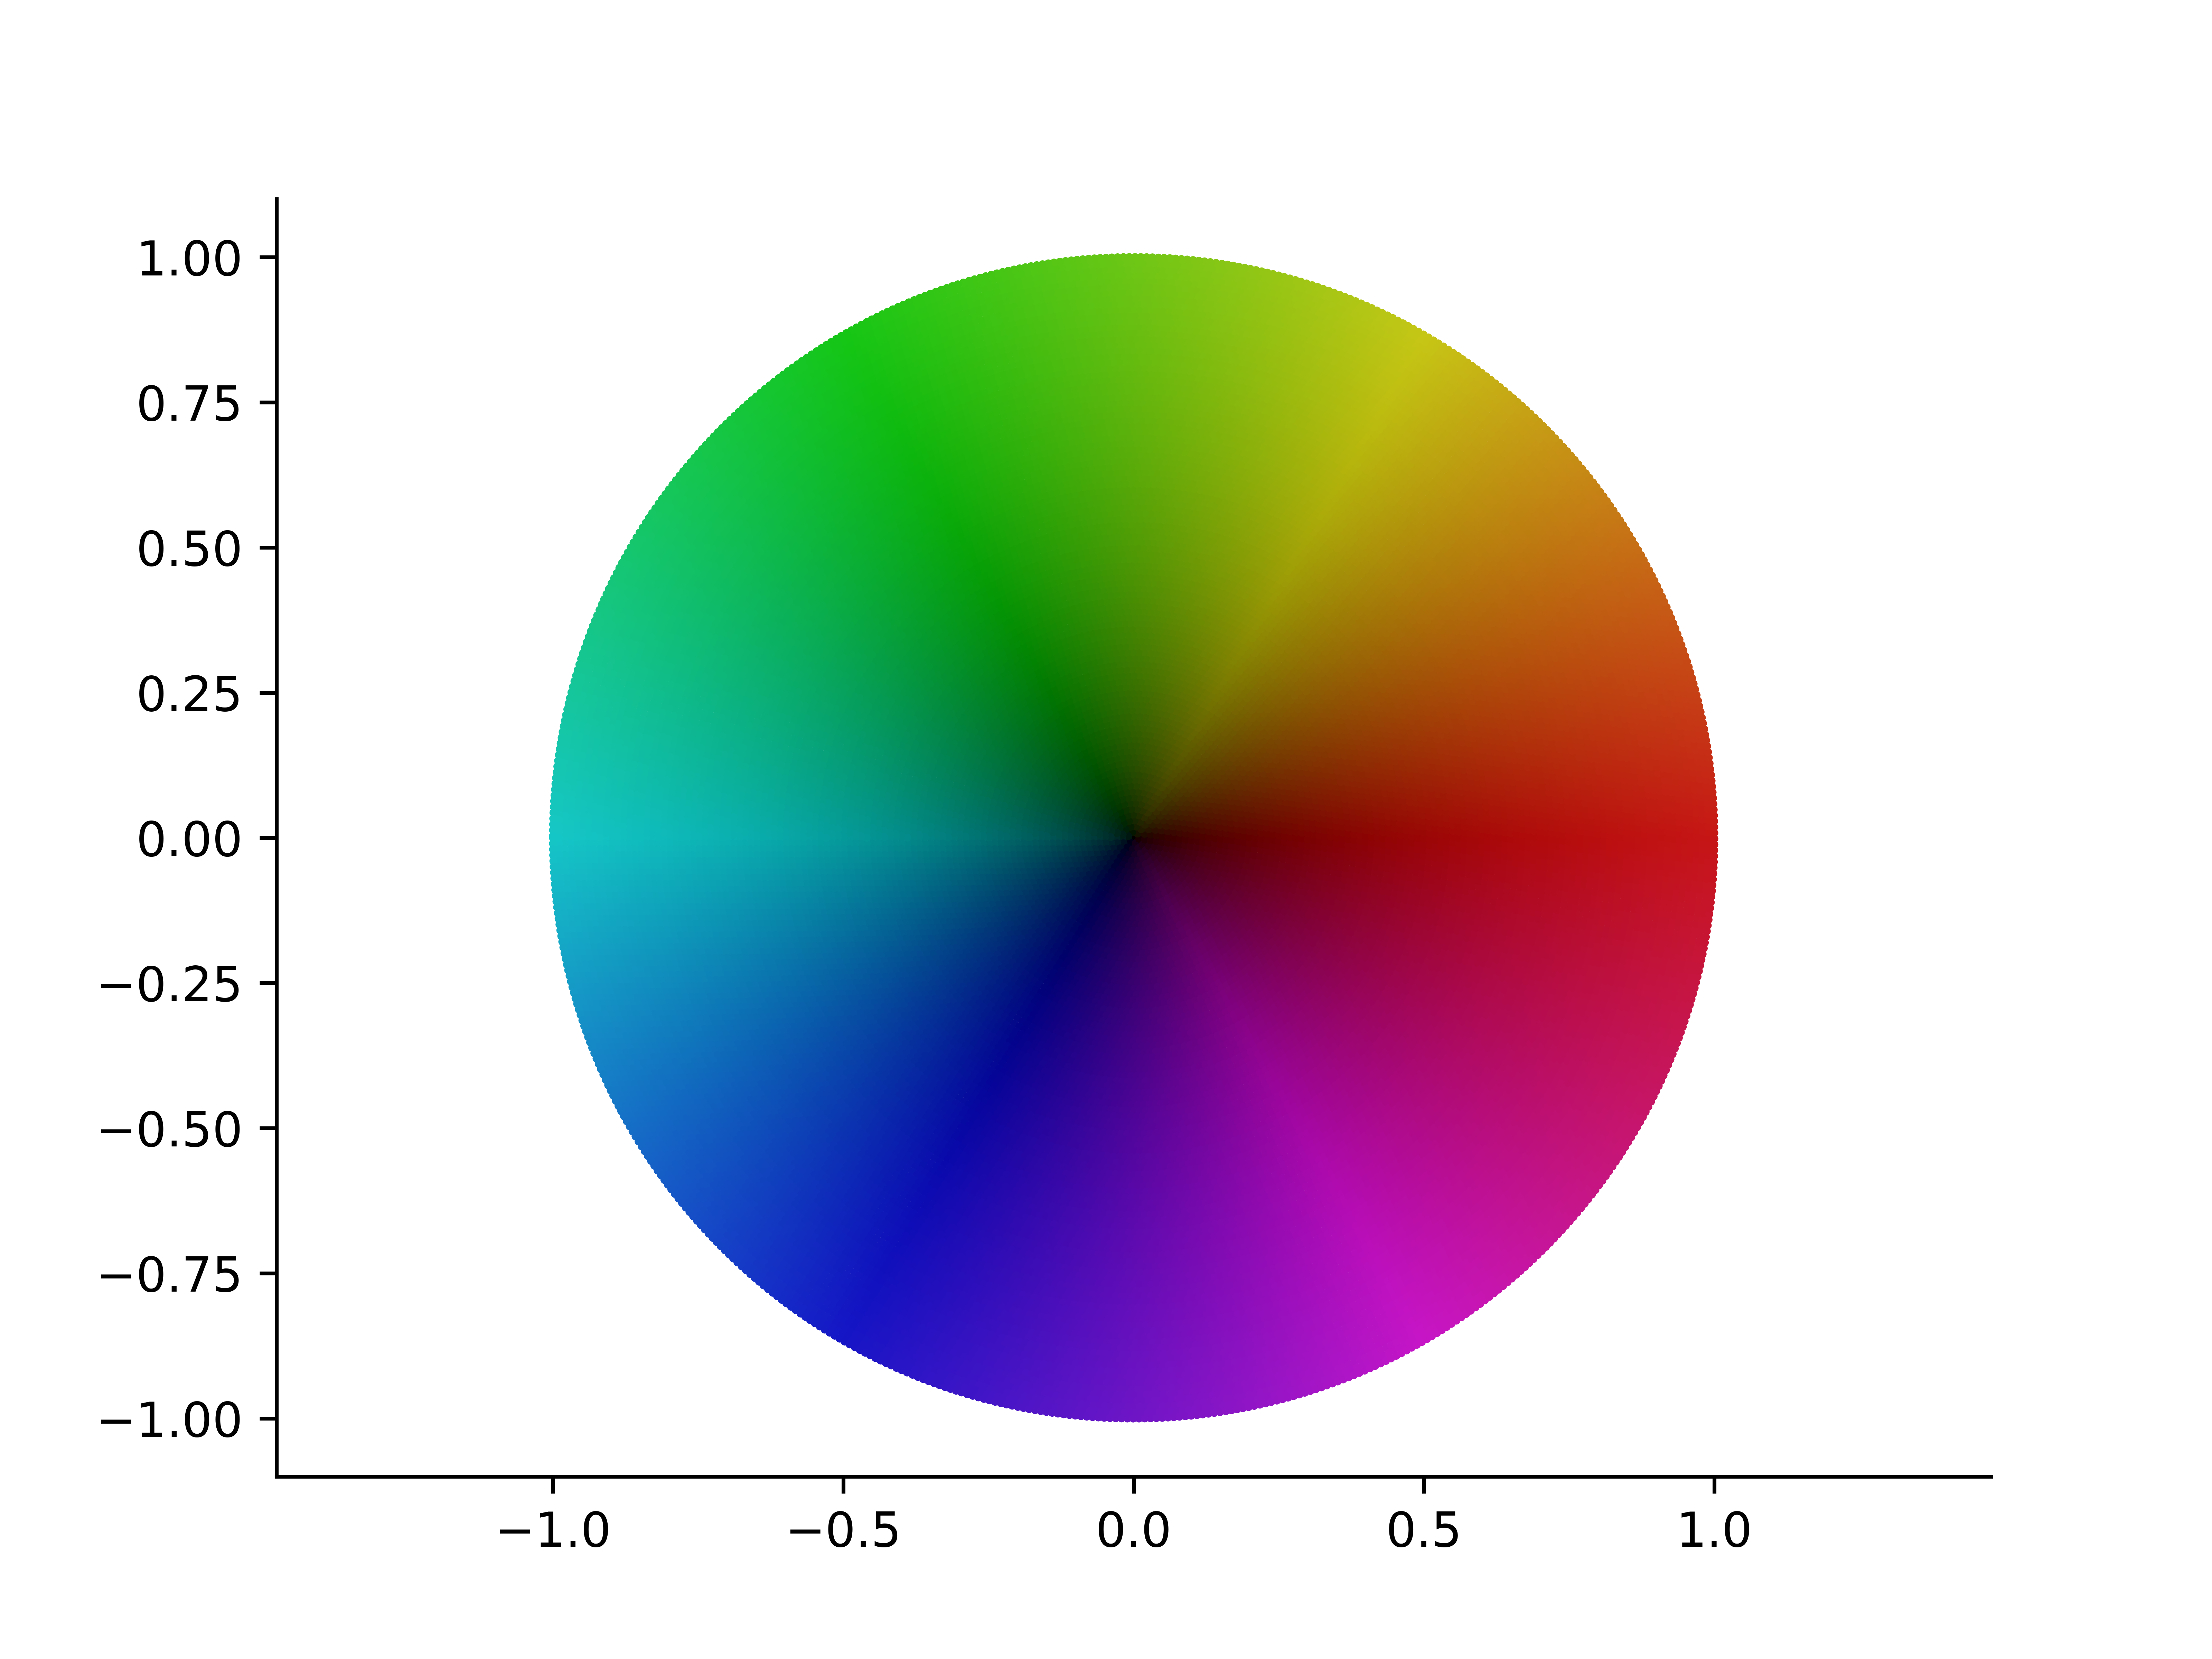
\includegraphics[width=0.49\textwidth]{../Aplicacion/3z.png}
    \hfill
    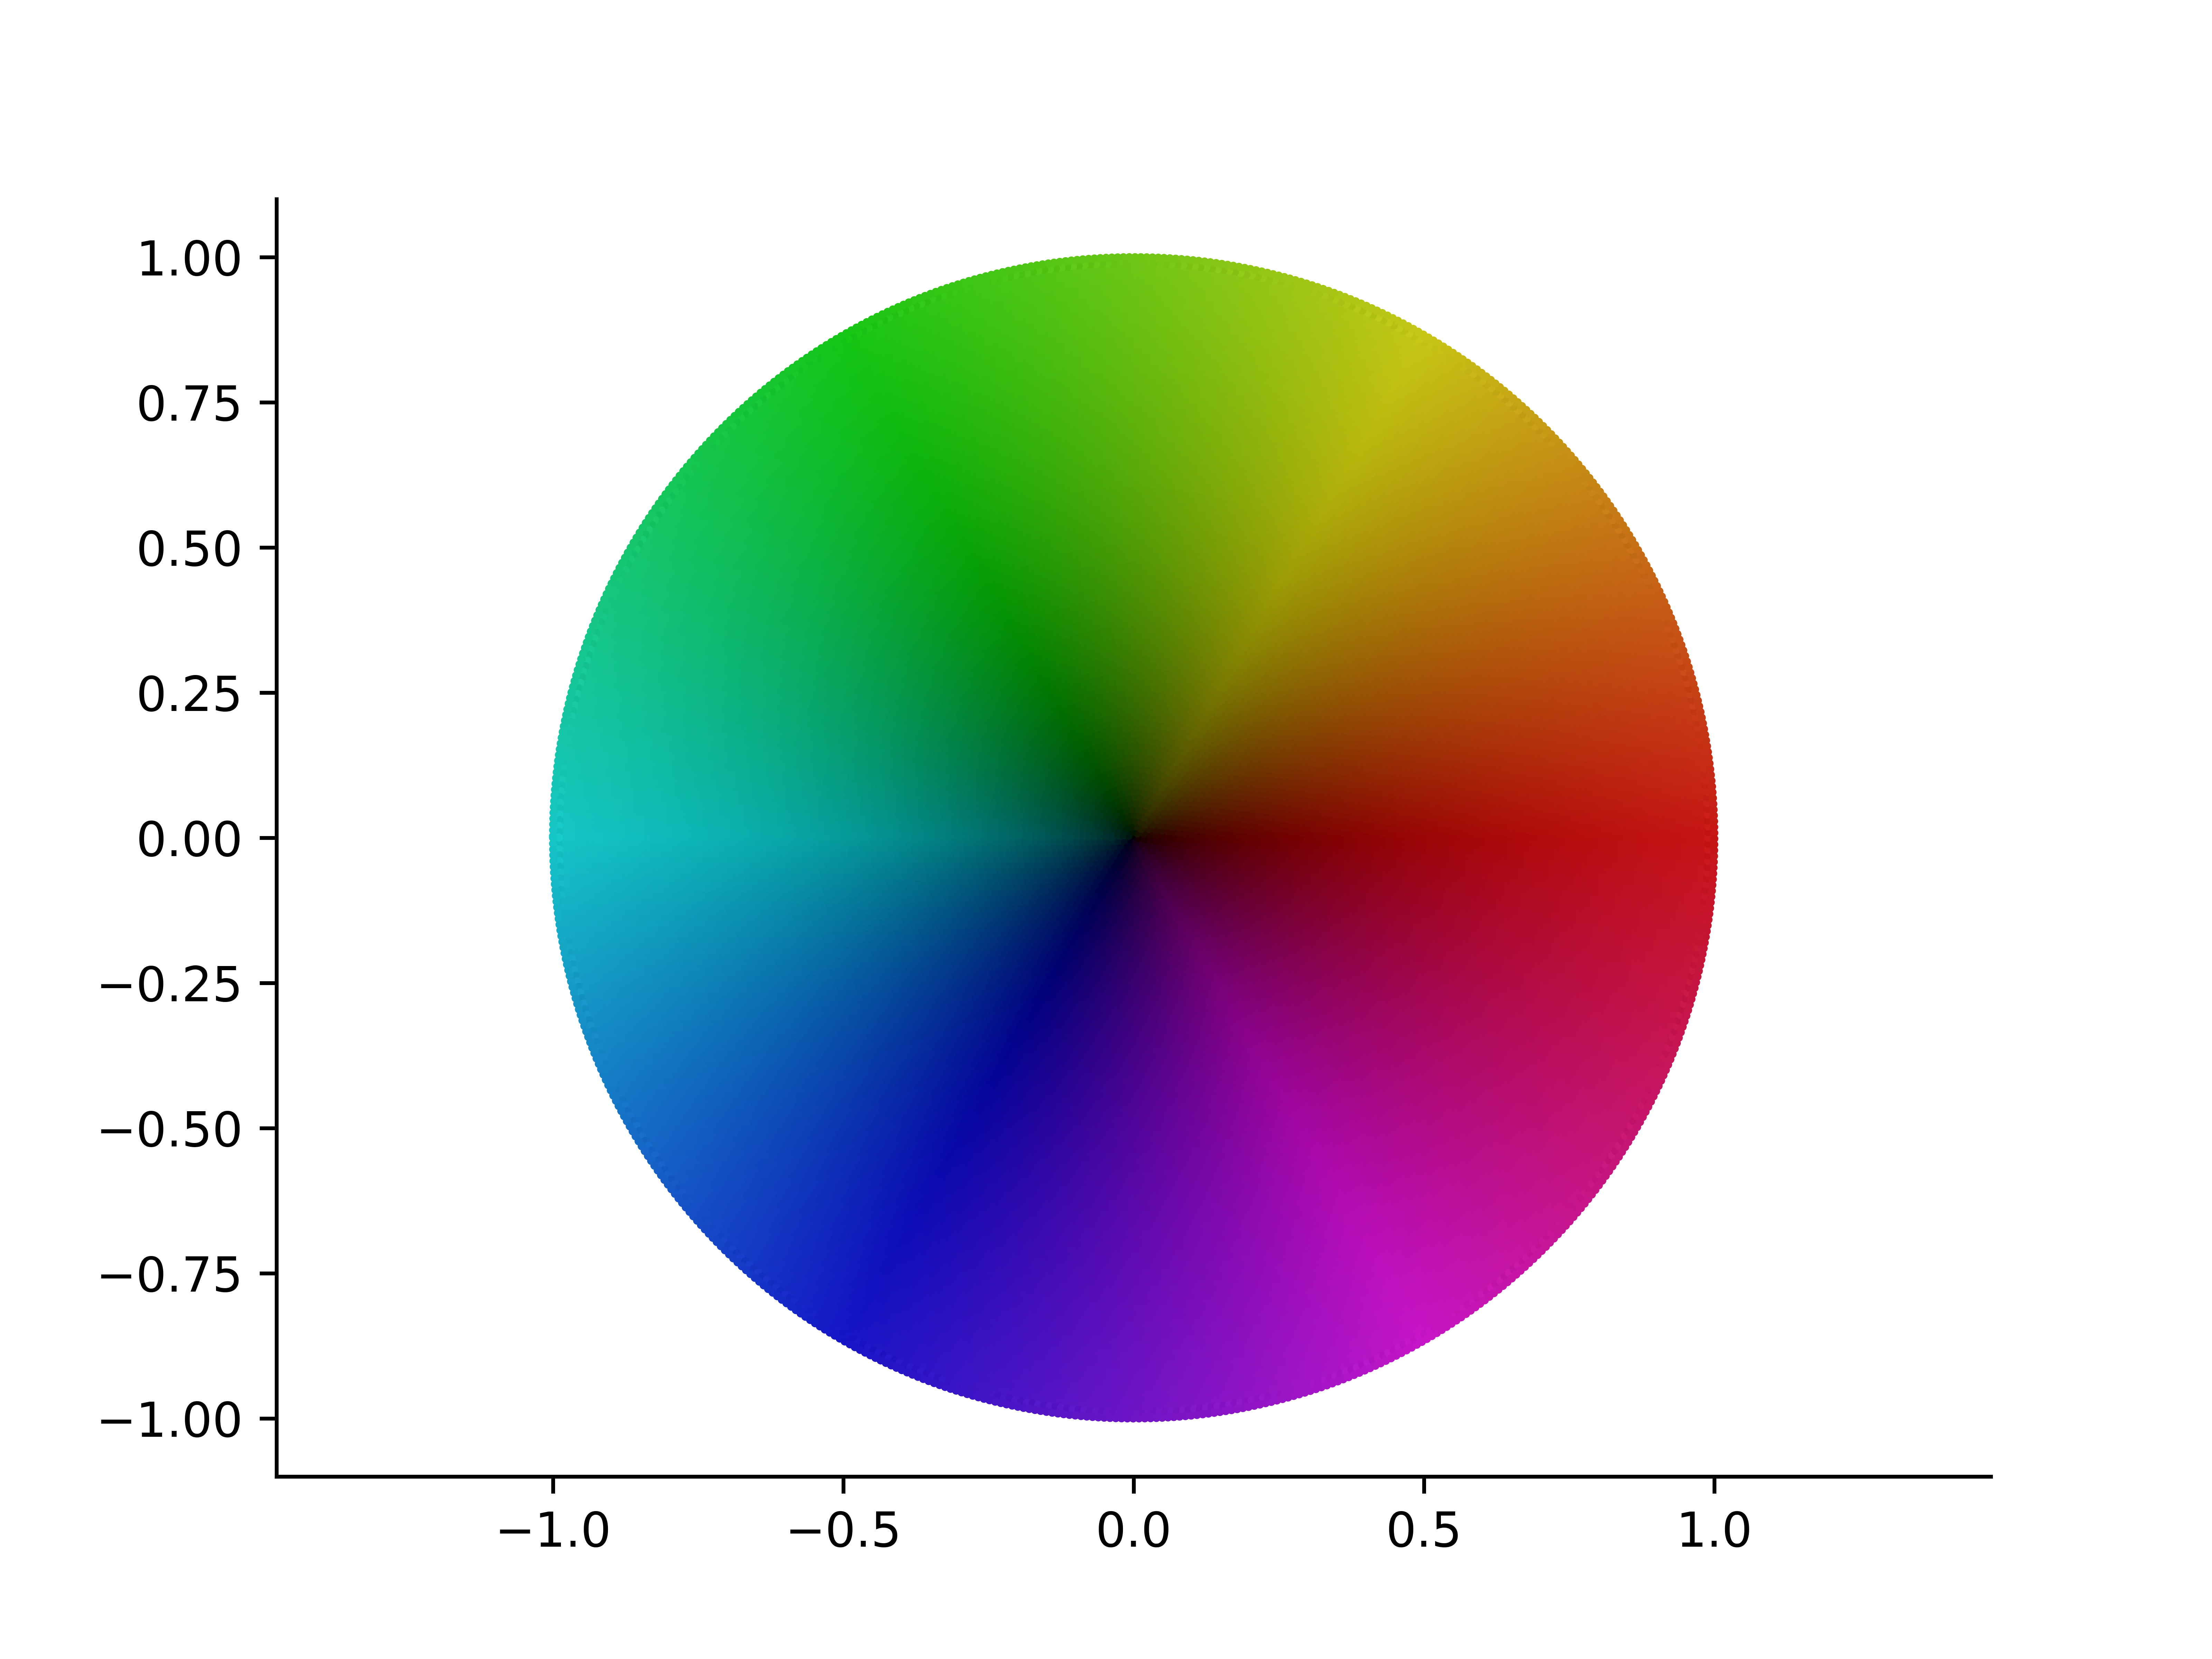
\includegraphics[width=0.49\textwidth]{../Aplicacion/3cos(t)+3isen(t).png}
    \caption{A la izquierda se muestra la representación de la función $f(z) = 3z$; a la derecha se muestra la extensión al disco de la función $f(t) = 3\cos(t) + 3i \sen(t)$.}
    \label{fig:comparacion2}
\end{figure}


\begin{figure}[h]
    \centering
    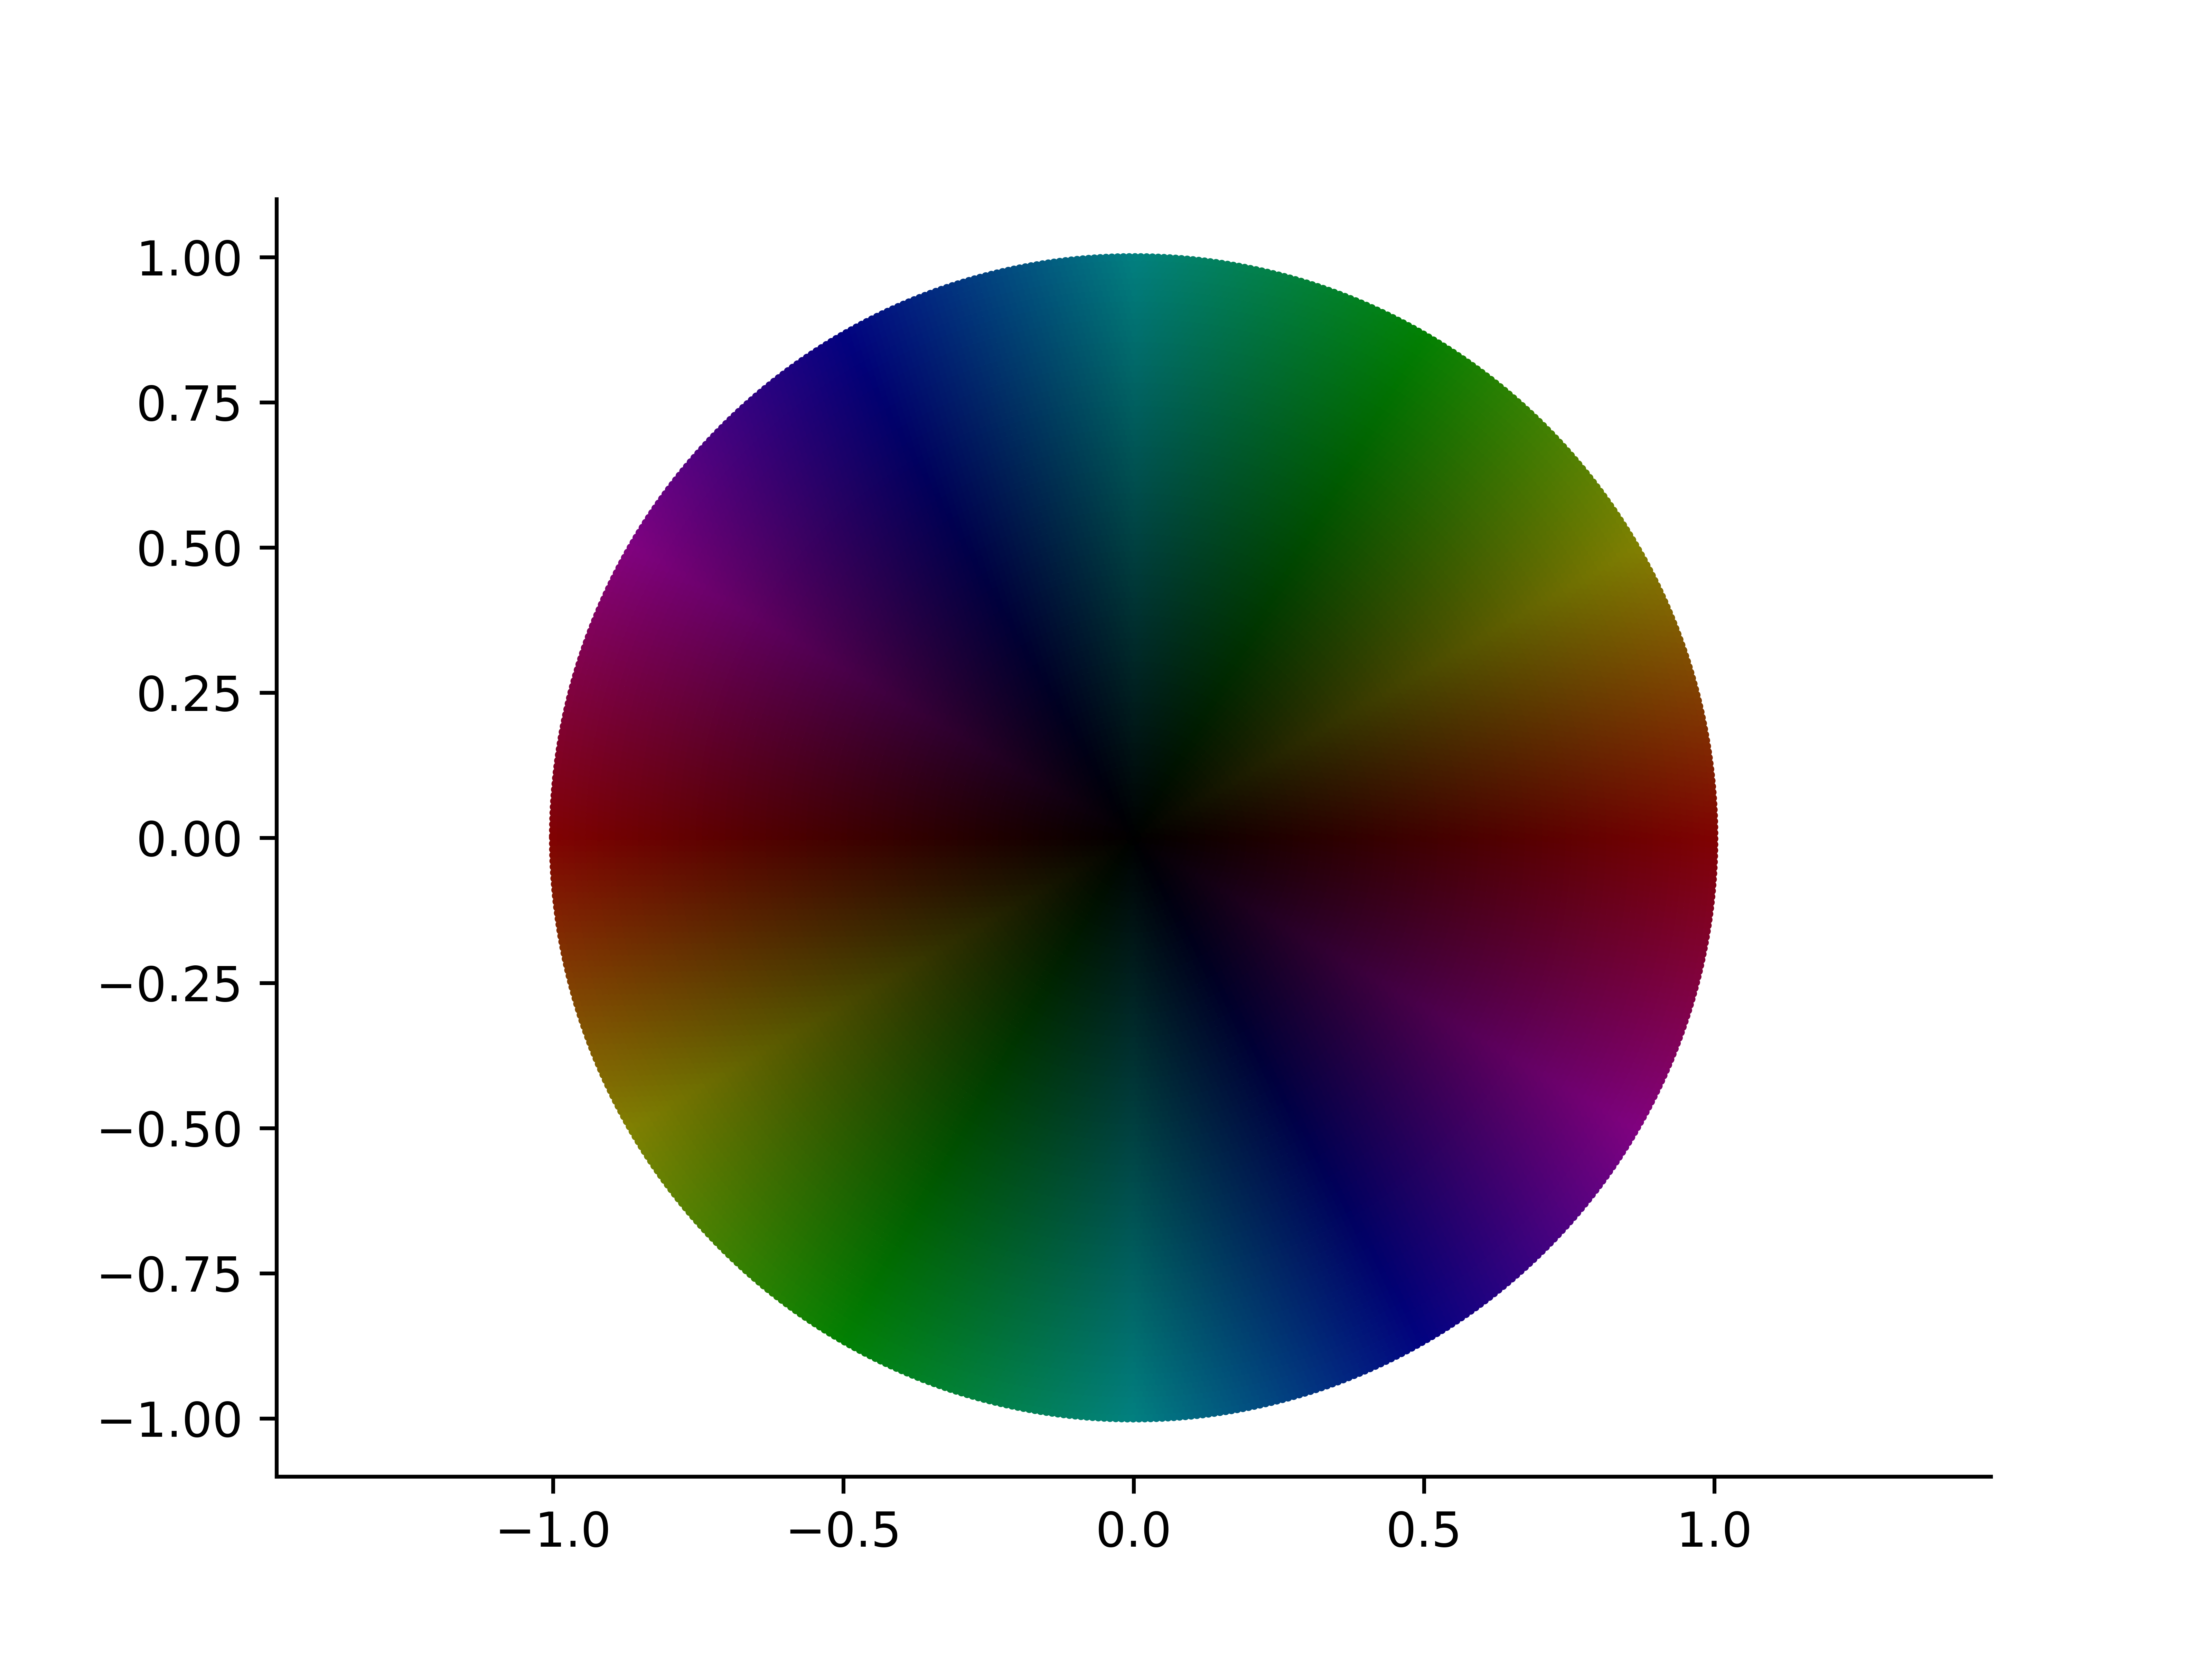
\includegraphics[width=0.49\textwidth]{../Aplicacion/z^2(2).png}
    \hfill
    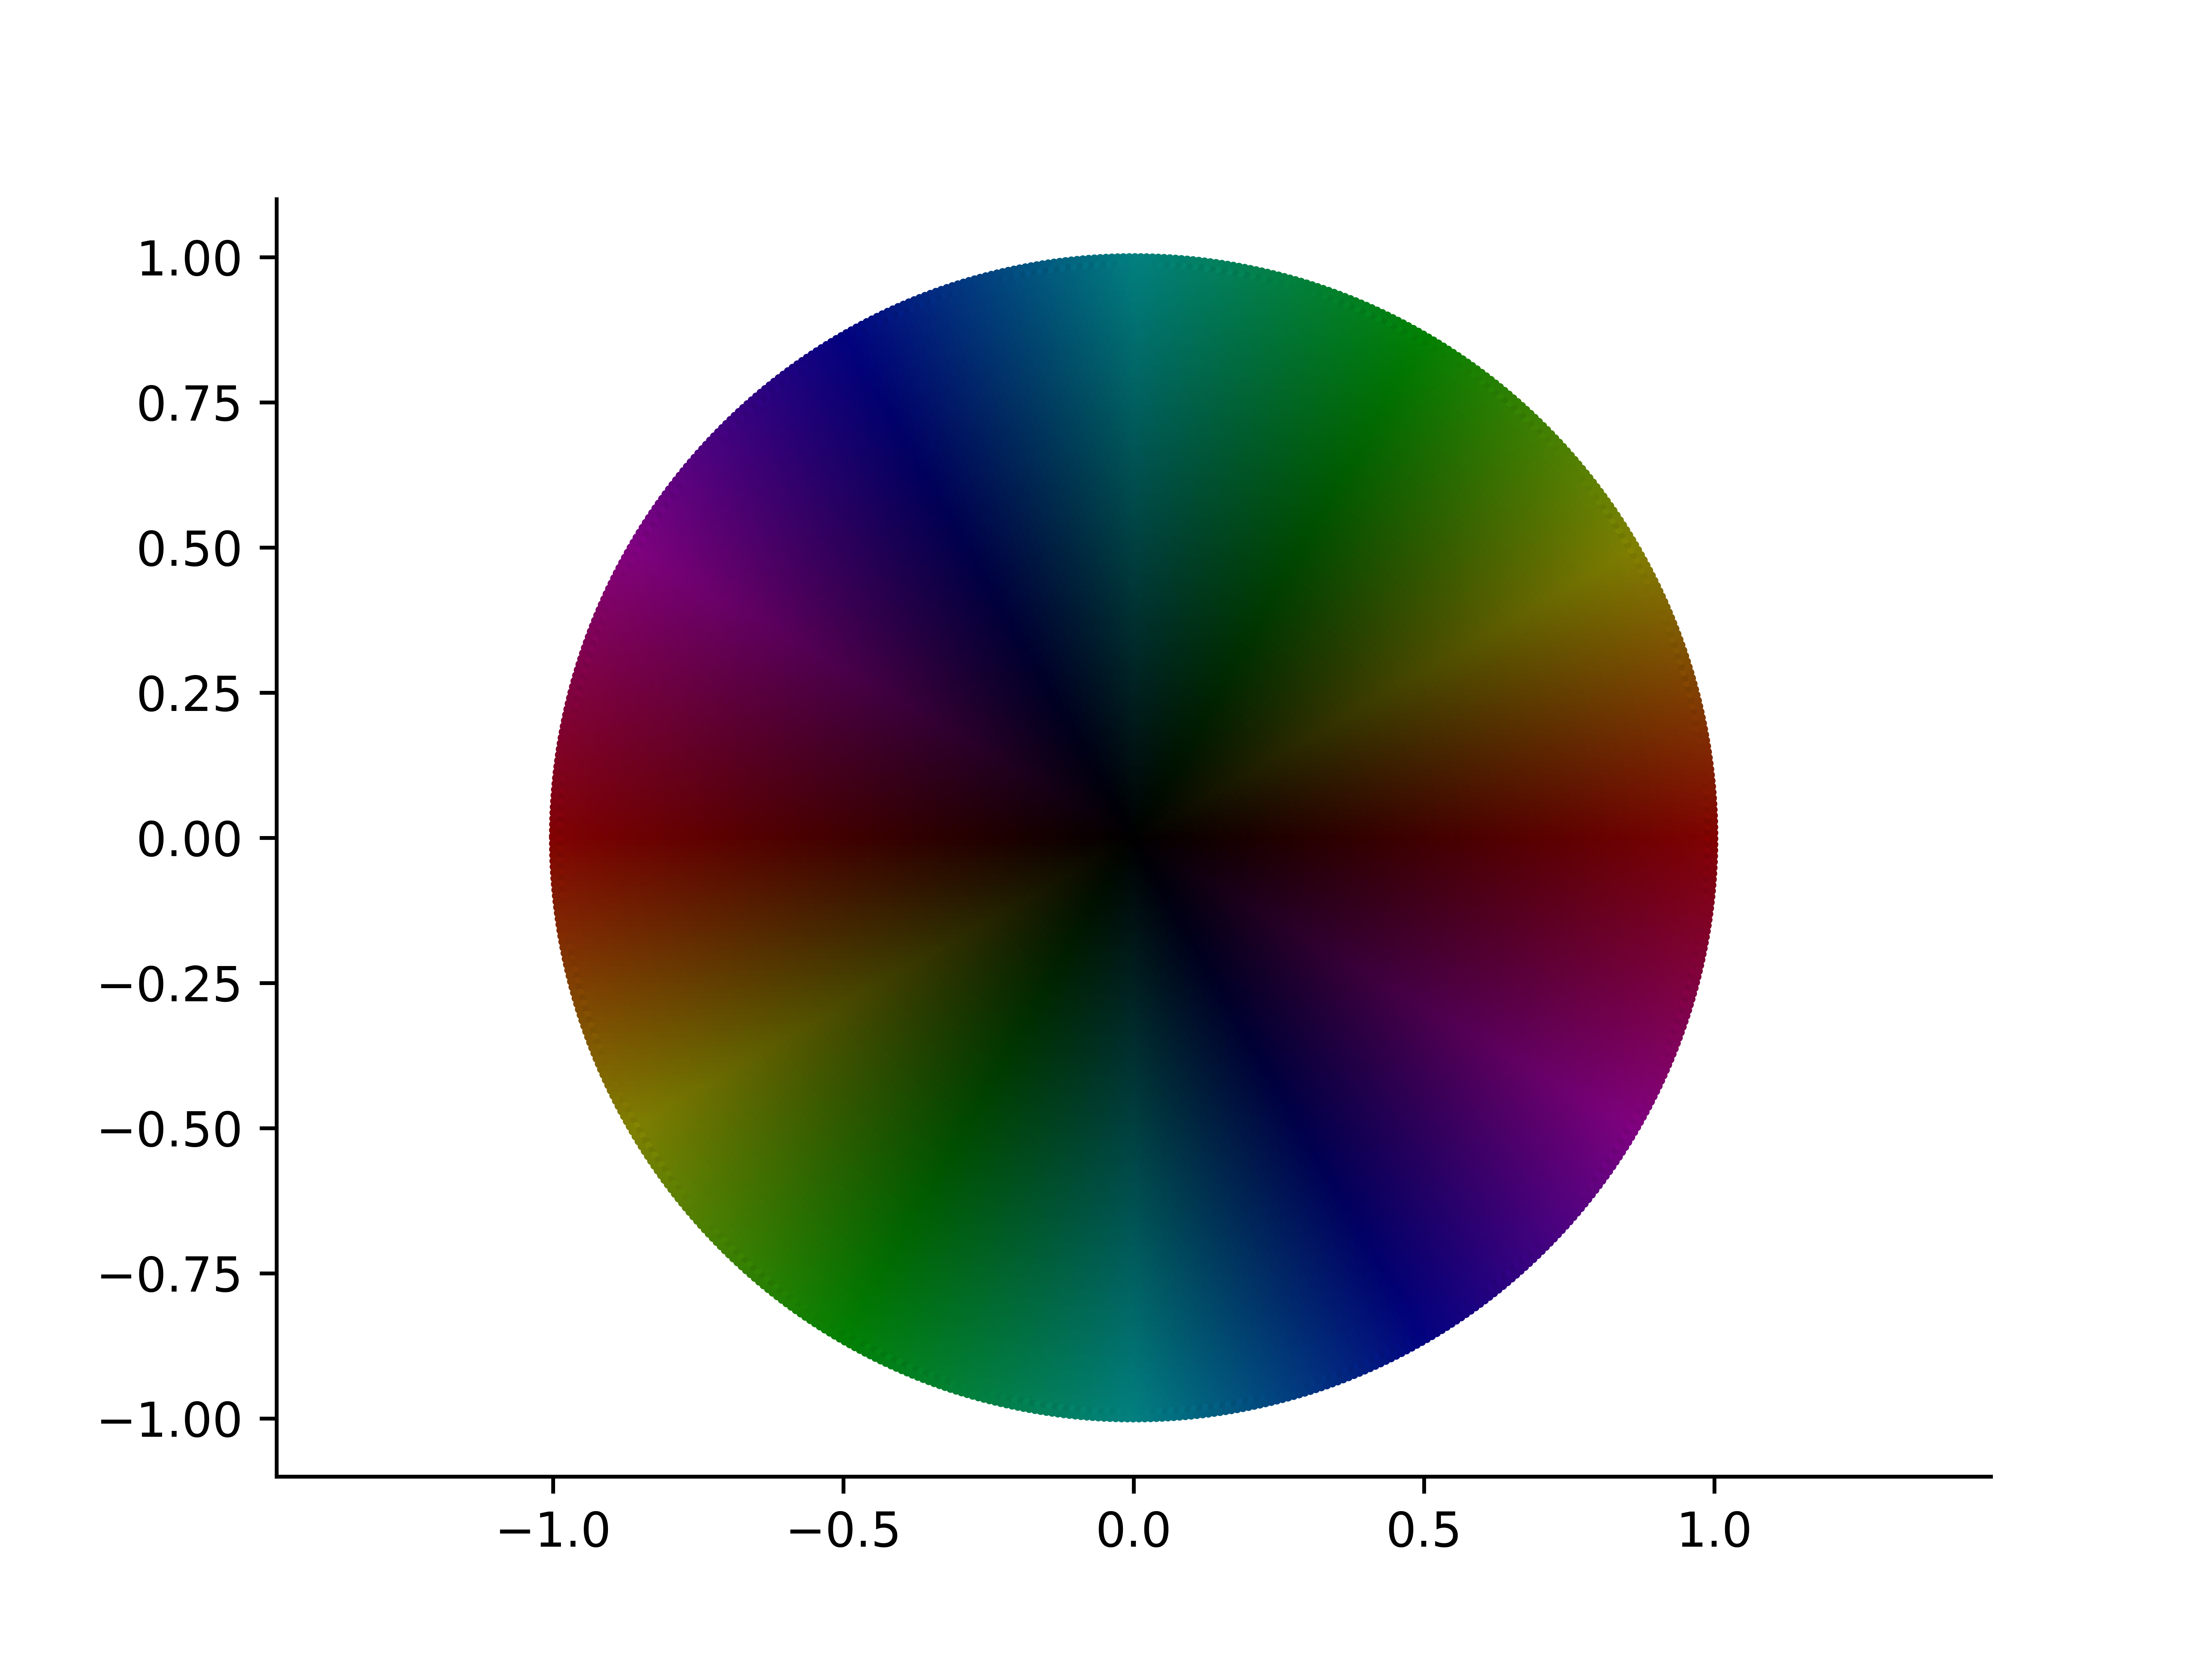
\includegraphics[width=0.49\textwidth]{../Aplicacion/cos^2(t)-sen^2(t)+(2cos(t)sen(t))i.png}
    \caption{A la izquierda se muestra la representación de la función $f(z) = z^2$; a la derecha se muestra la extensión al disco de la función $f(t) = \cos^2(t) - \sen^2(t) + i (2 \cos(t) \sen(t))$.}
    \label{fig:comparacion3}
\end{figure}


\begin{figure}[h]
    \centering
    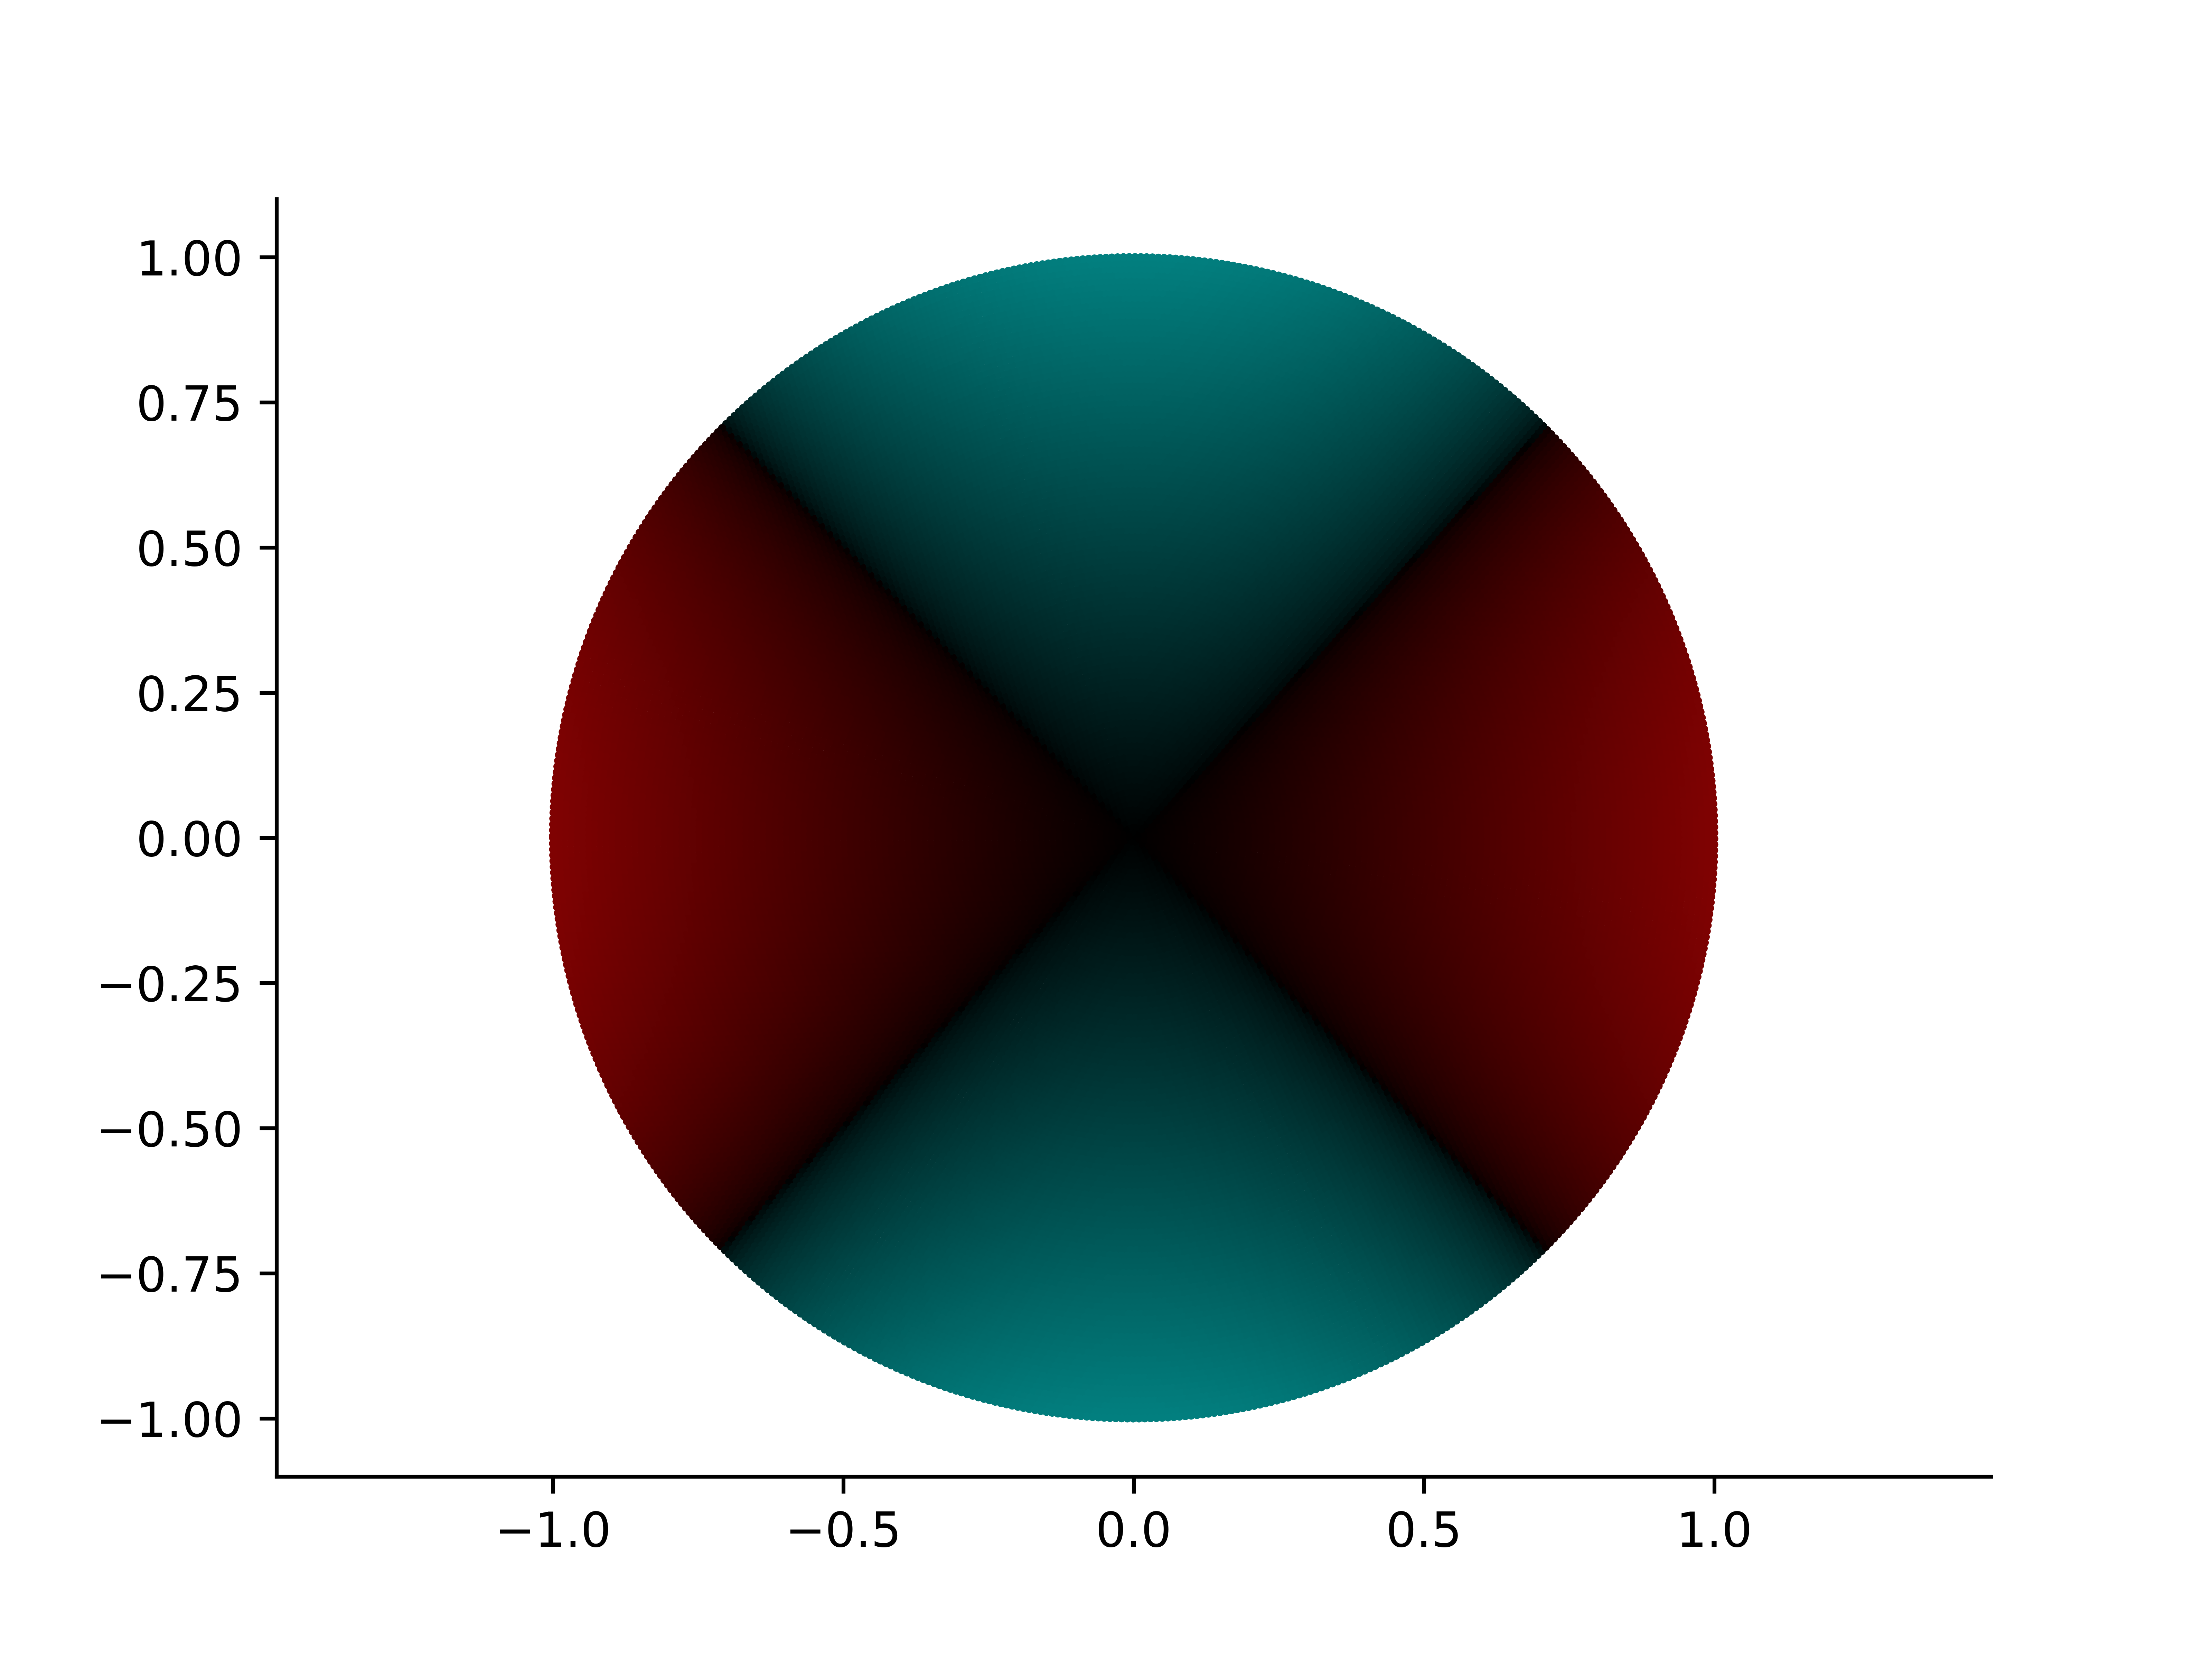
\includegraphics[width=0.49\textwidth]{../Aplicacion/z^2(3).png}
    \hfill
    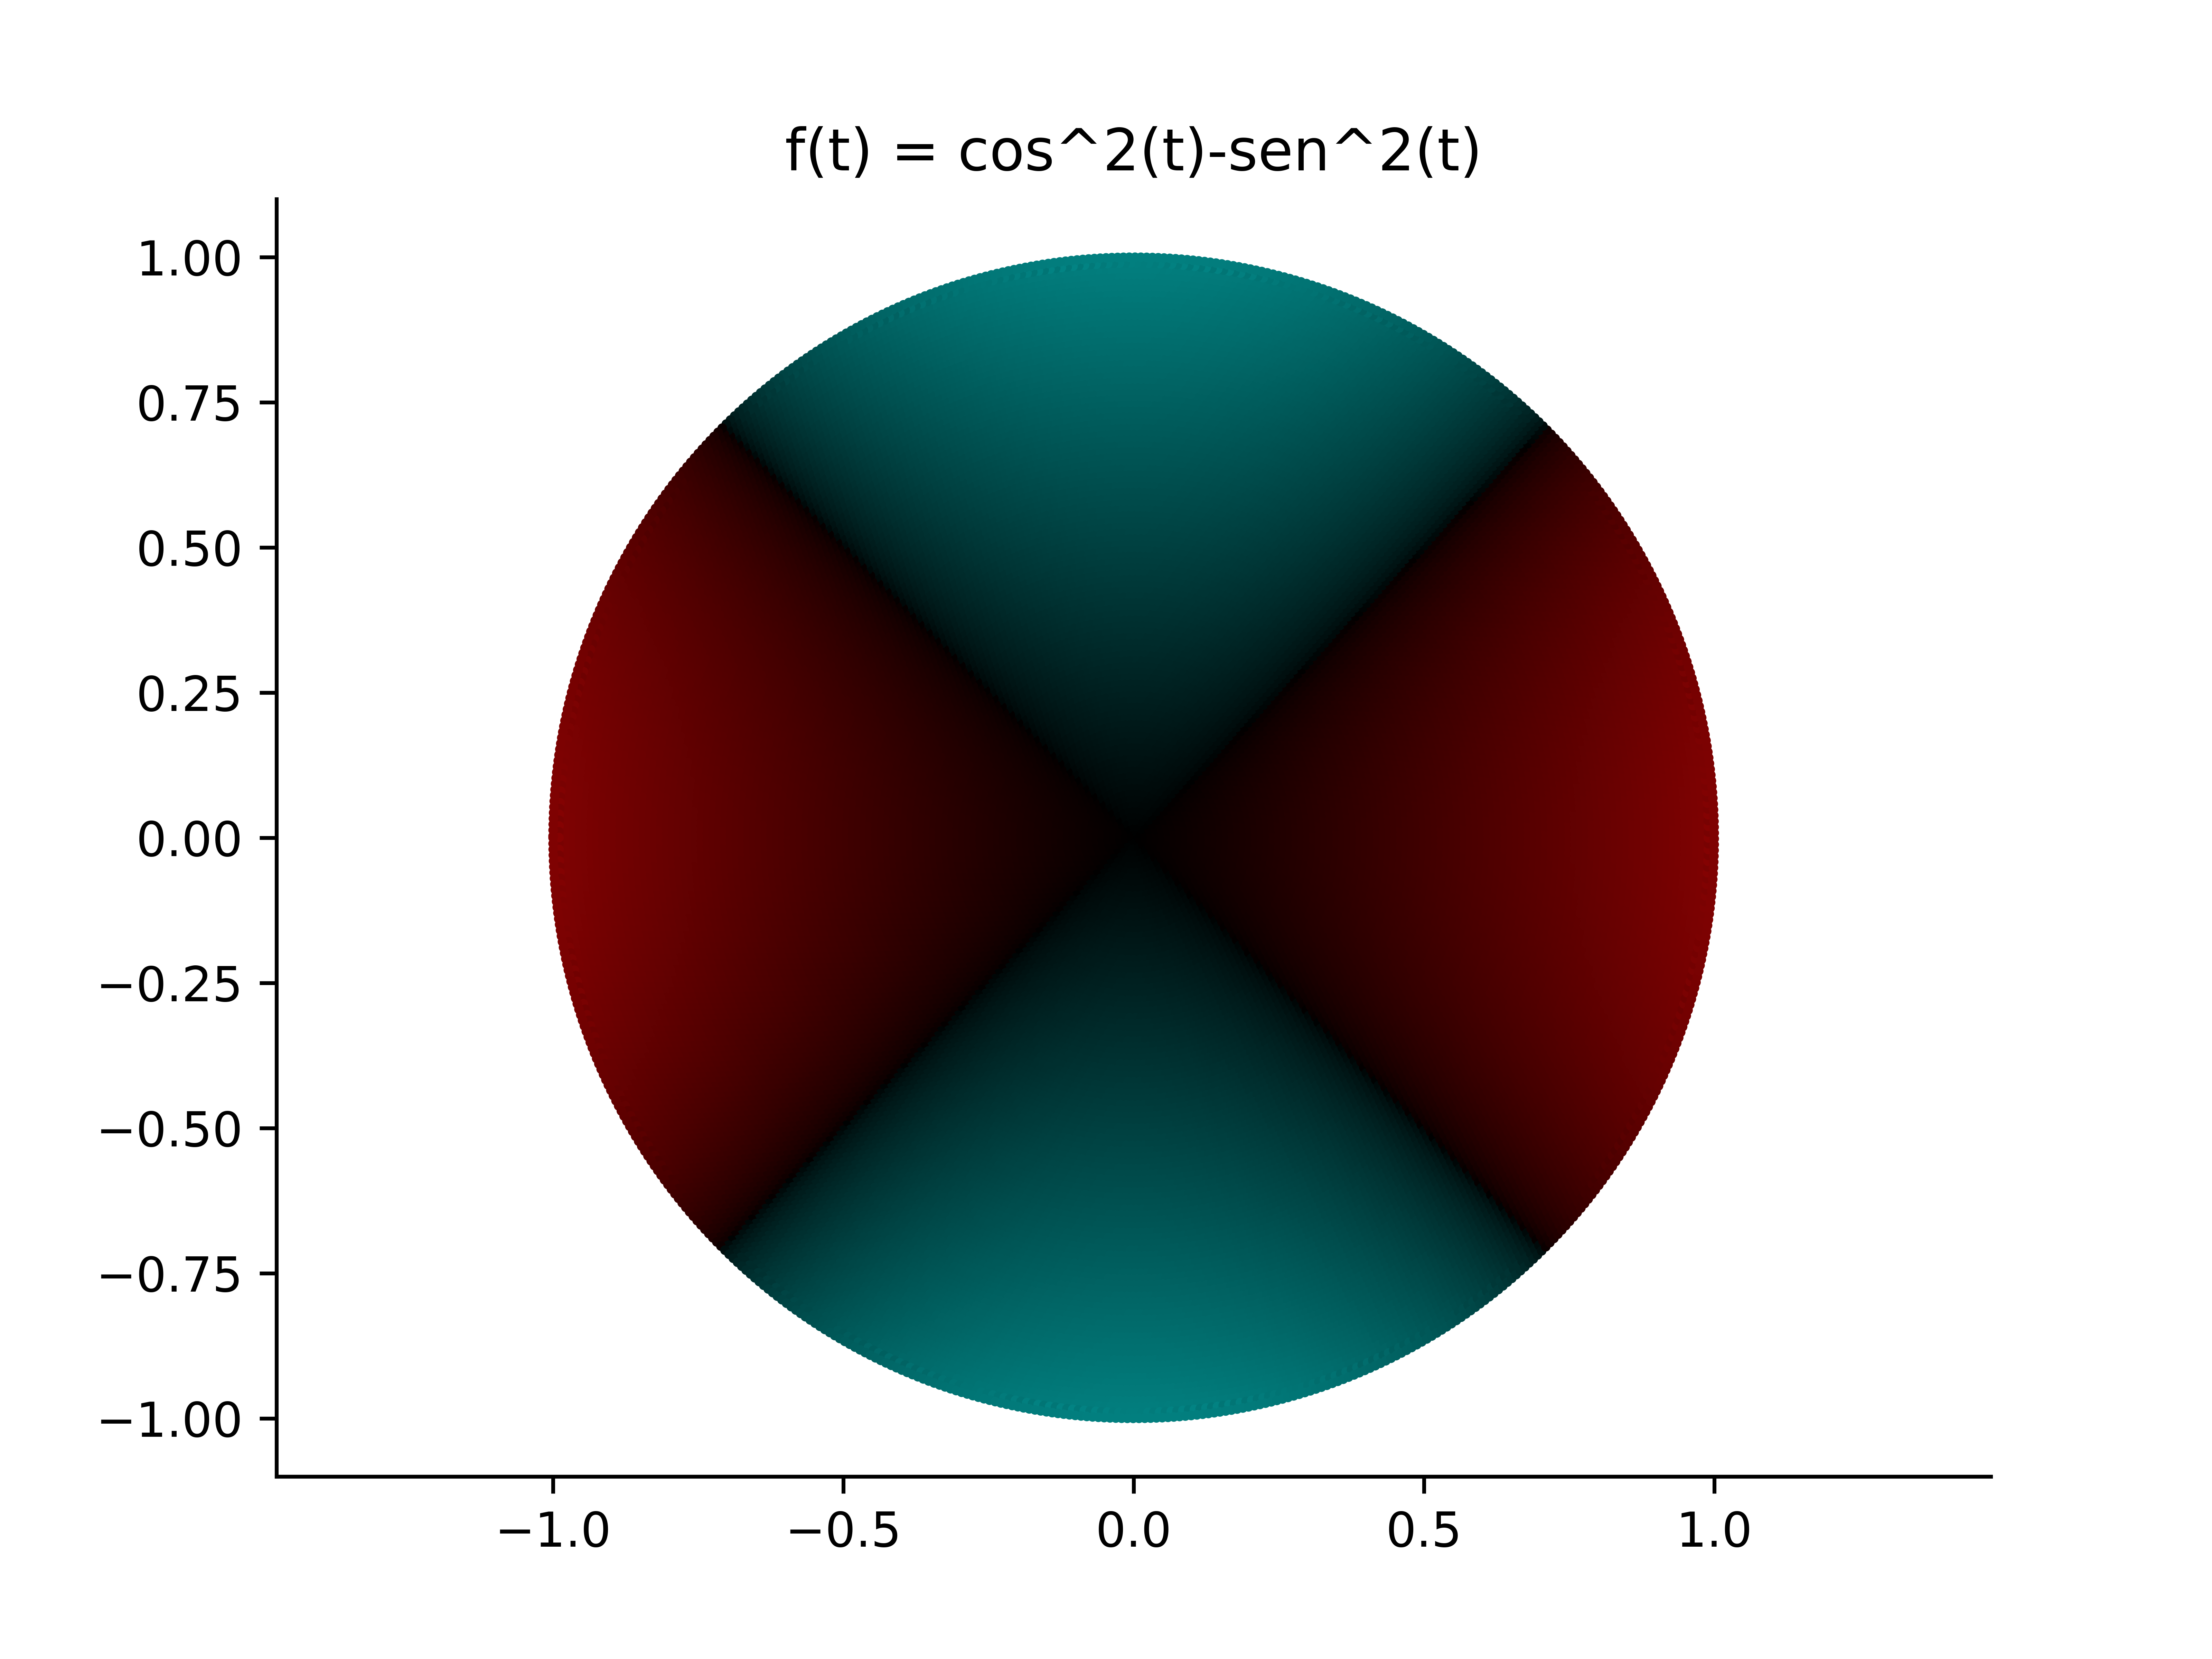
\includegraphics[width=0.49\textwidth]{../Aplicacion/cos^2(t)-sen^2(t).png}
    \caption{A la izquierda se muestra la representación de la función $f(z) = \Re (z^2)$; a la derecha se muestra la extensión al disco de la función $f(t) = \cos^2(t) - \sen^2(t)$.}
    \label{fig:comparacion4}
\end{figure}

Esta misma comprobación se puede llevar a cabo mediante la última funcionalidad de la aplicación que permite representar la diferencia de funciones. Por lo tanto, si el cálculo de la integral de Poisson fuera perfecto, el dibujo resultante sería negro en su totalidad. \\

Como hemos comentado previamente, $f$ ha de ser continua para que se pueda extender con continuidad al disco cerrado. Pero, ¿qué pasa cuando no lo es? El resultado será una función con parte real e imaginaria armónicas en el interior (no necesariamente una conjugada de la otra) pero que no se puede prolongar con continuidad a la frontera, como es lógico. Además, si $f$ es continua a trozos, la función que se obtiene a partir de ella es armónica y continua en los puntos del borde donde lo sea $f$. \\

\begin{figure}[h]
    \centering
    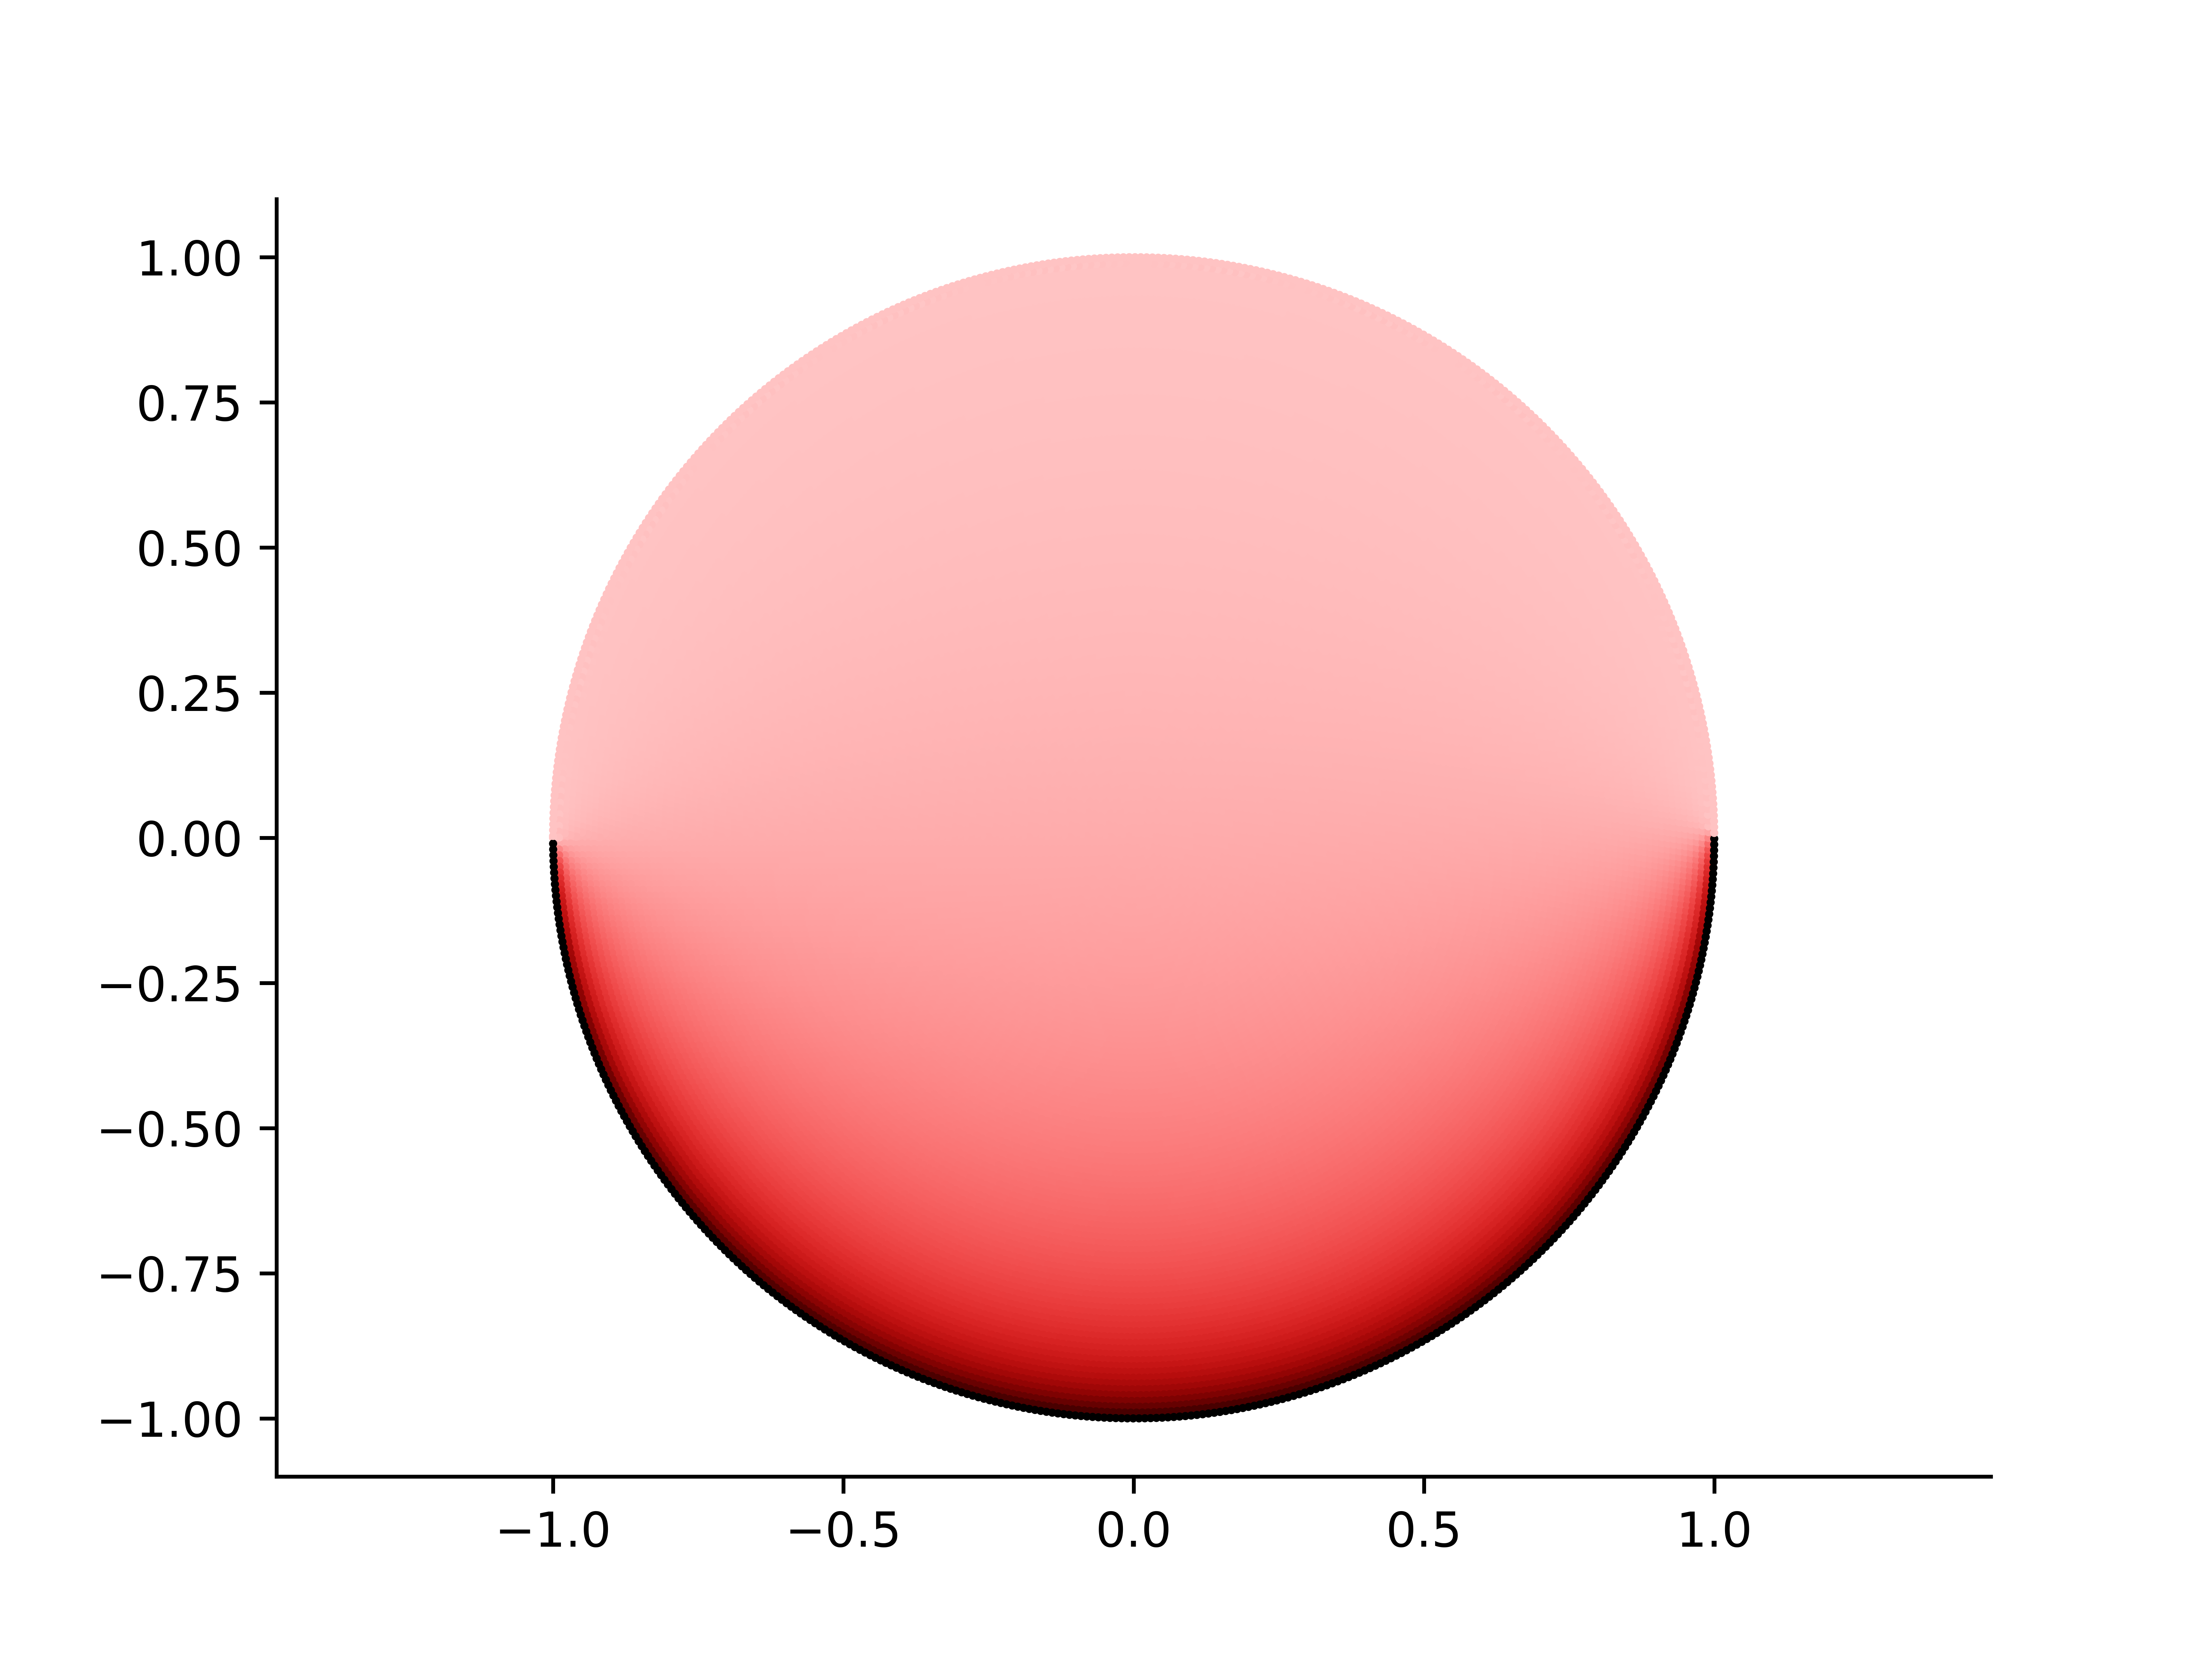
\includegraphics[width=0.49\textwidth]{../Aplicacion/atrozos.png}
    \hfil
    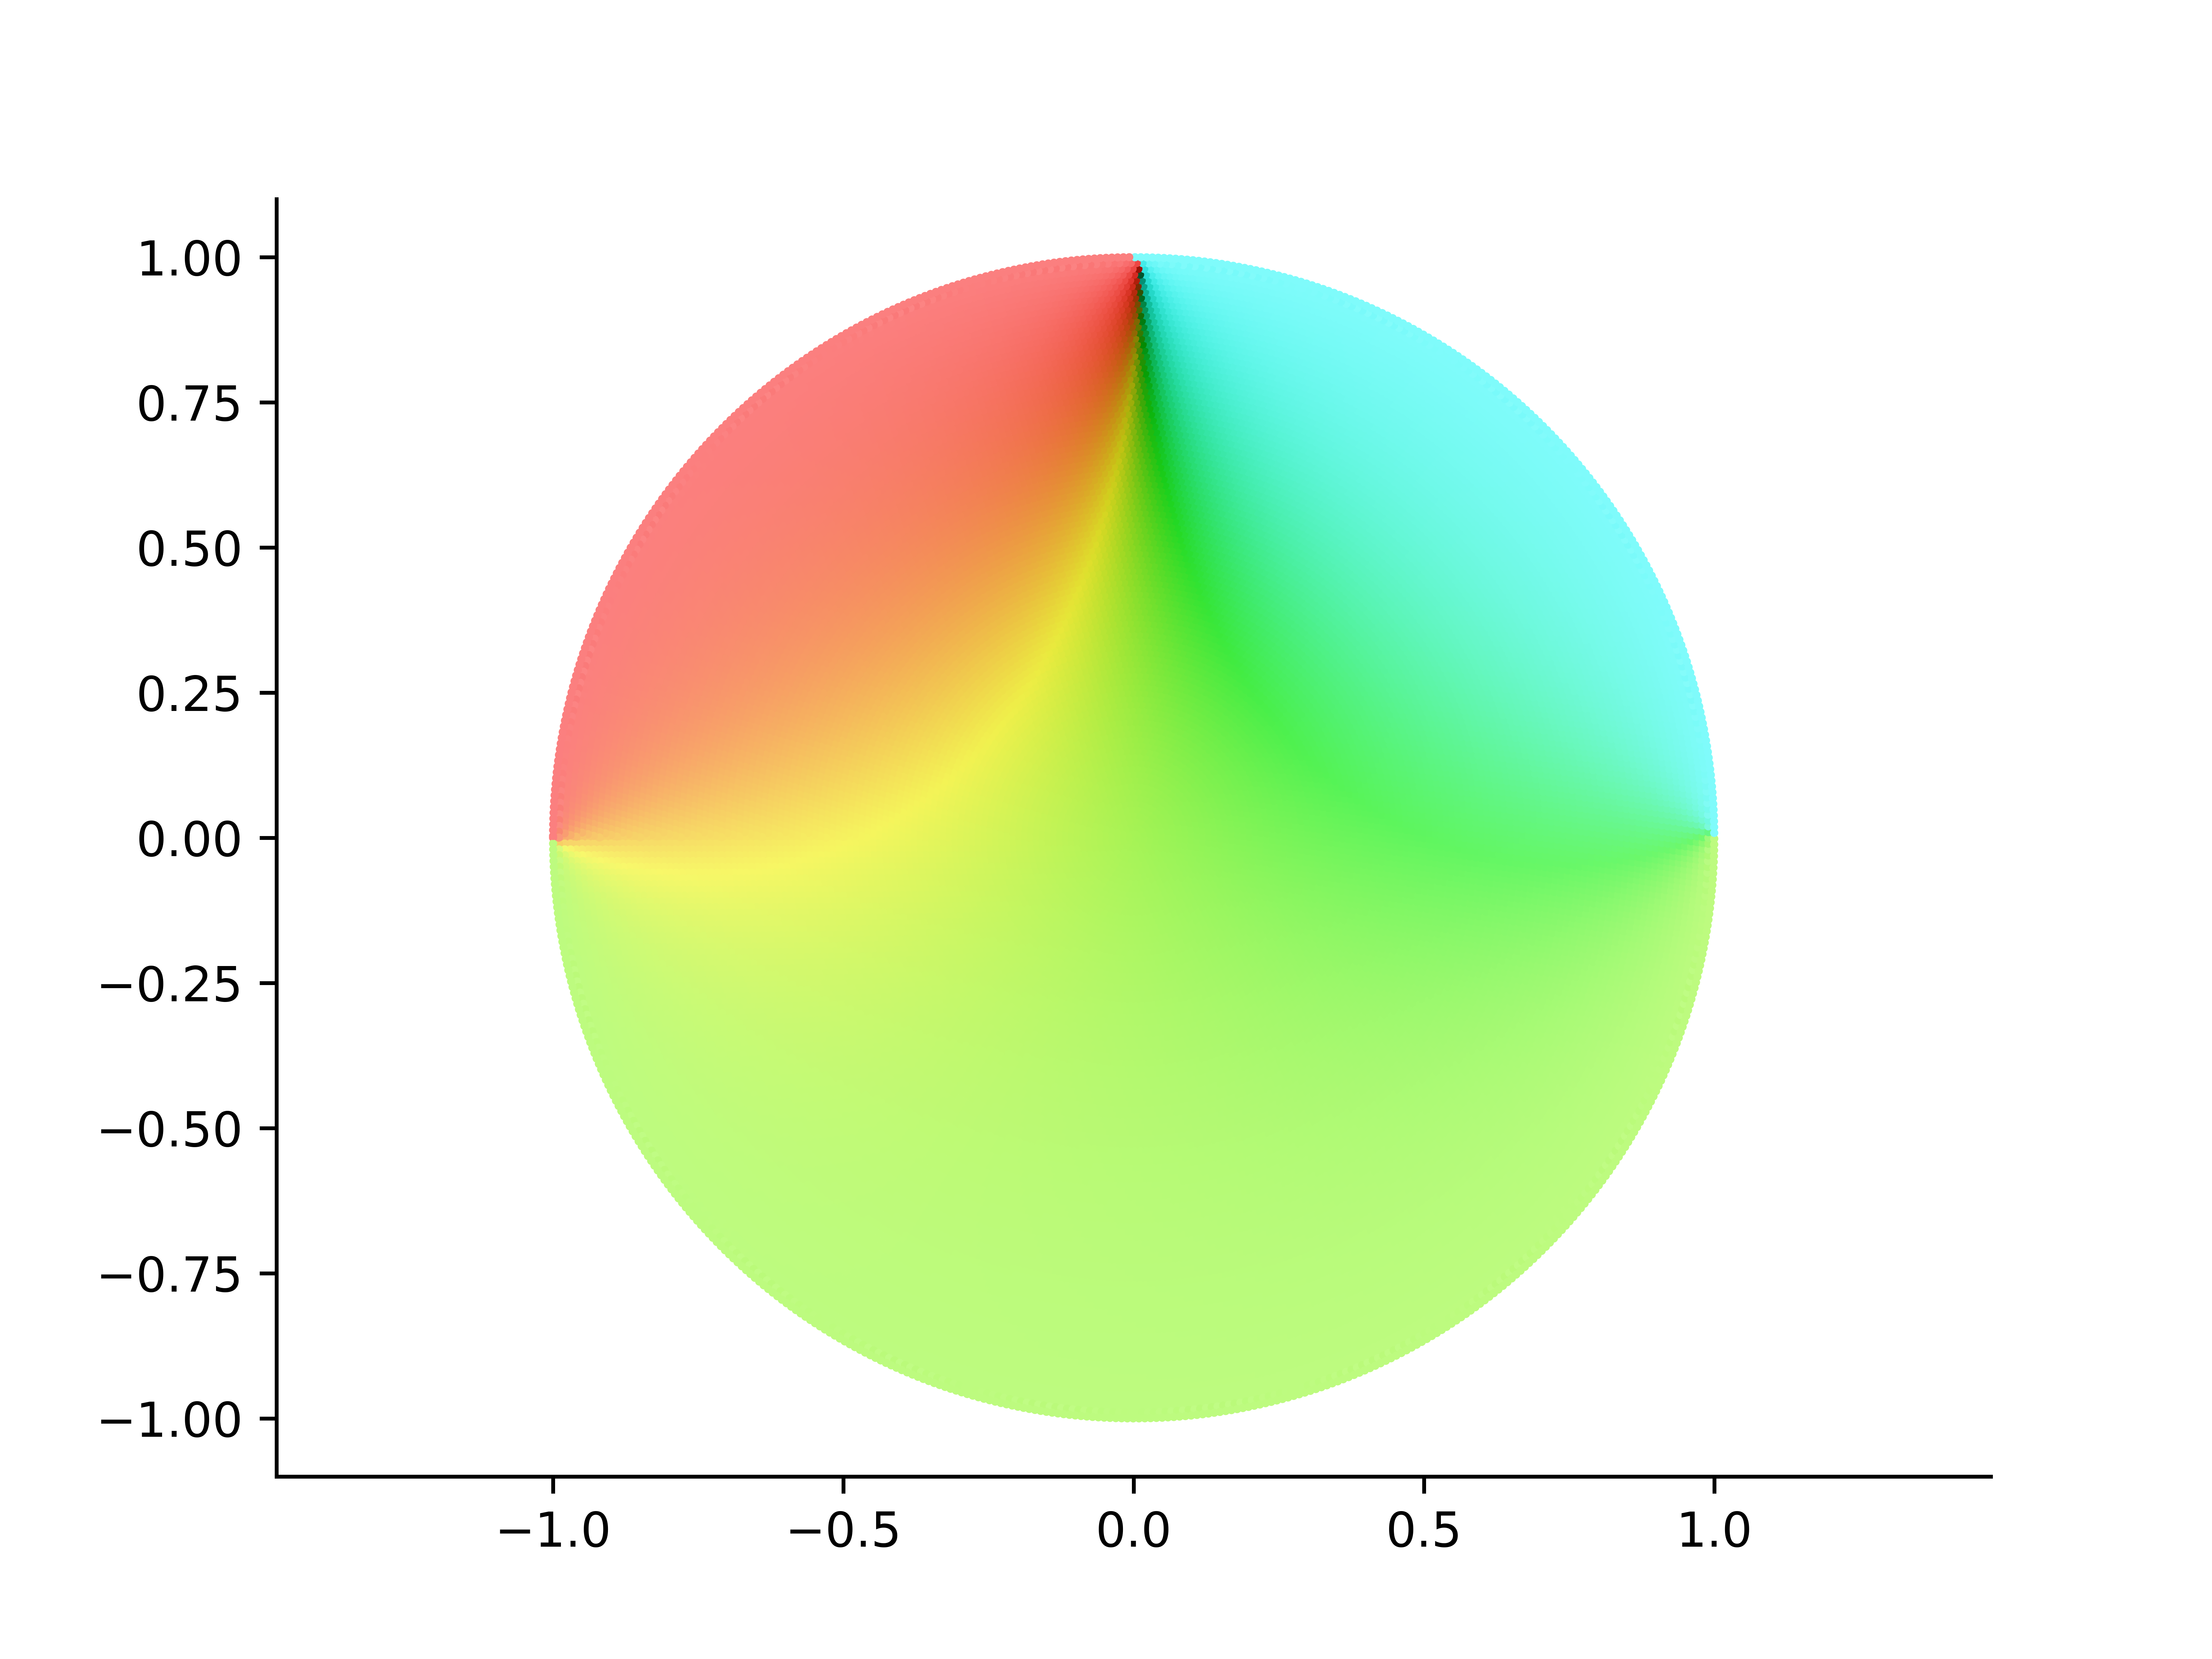
\includegraphics[width=0.49\textwidth]{../Aplicacion/atrozos(2).png}
\caption{A la izquierda se muestra la representación de la función $f(t) = 0$ si $- \pi < t < 0$ y $f(t) = 100$ si $0 \leq t \leq \pi$; a la derecha se muestra la representación de la función $f(t) = 20i$ si $- \pi < t < 0$, $f(t) = -20$ si $0 \leq t < \frac{\pi}{2}$ y $f(t) = 20$ si $\frac{\pi}{2} \leq t \leq \pi$.}
    \label{fig:atrozos}
\end{figure}

